\documentclass[11pt]{book}
\usepackage{graphicx}
\usepackage[dvipsnames]{color}
\usepackage[hidelinks]{hyperref}
\usepackage[square,numbers]{natbib}
%pPara poder modificar los margenes
\usepackage{geometry}
\geometry{
	a4paper,
	total={170mm,257mm},
	left=30mm,
	right=30mm,
	top=30mm,
	bmargin=30mm,
}
%Para usar el español
\usepackage[spanish]{babel}
\usepackage[utf8]{inputenc}
\usepackage{lscape}
\usepackage{hyperref}
\bibliographystyle{plain}
\begin{document}
	%Portada
	\begin{titlepage}
		\centering
		{
\includegraphics[width=0.8\textwidth]{logo}\par}
		\vspace{1cm}
		{\Large Facultad de Informática \par}
		\vspace{1cm}
		{\Huge Aplicación web de soporte al Aprendizaje-Servicio: gestión de ofertas y demandas de servicio\par}
		\vspace{1cm}
		{\Huge Web application for supporting Service Learning: management of service offers and service requests \par}
		\vspace{2cm}
		{\textbf\Large Autores \par}
		{\Large Daniela-Nicoleta Boldureanu (Grado en Ingeniería del Software)\par}
		{\Large Victoria Gnatiuk Romaniuk (Grado en Ingeniería Informática)\par}
		{\Large Jesús Sánchez Granado (Grado en Ingeniería Informática)\par}
		\vspace{1cm}
		{\textbf\Large Directores \par}
		{\Large Simon Pickin \par}
		{\Large Manuel Montenegro Montes \par}
		\vspace{2cm}
		{\Large Curso 2020/2021 \par}
	\end{titlepage}
	
<<<<<<< HEAD
	\tableofcontents
	\newpage
	\listoffigures
	
	\chapter{Introducción}
	El objetivo de este \textit{Trabajo de Fin de Grado} (TFG) es retomar la idea de creación de una comunidad web de proyectos ApS (\emph{Aprendizaje-Servicio}) empezada a nuestro saber, en el año 2004 por Emmanuel Parmentier en su (\emph{Proyecto Fin de Carrera}) PFC. Otros trabajos después siguieron esta trayectoria y el último de ellos fue el TFG de David Jiménez del Rey, este es el proyecto que nosotros continuamos en nuestro TFG. Estos proyecto precedentes se detalla más adelante en el capítulo \ref{cap:cont-motidvacion}. El proyecto objetivo en cuestión consiste en la creación de una plataforma web que permita crear un entorno digital en el que las empresas, principalmente del sector público, y las universidades desarrollen actividades de labor social que ayuden a los alumnos a desarrollar de forma práctica lo aprendido en el aula y a moldearles como ciudadanos éticos y solidarios.
	
	\section{Antecedentes}
	Este trabajo parte del TFG de David Jiménez del Rey, que se desarrolló en la \emph{Universidad Nacional de Educación a Distancia} (UNED) bajo la tutela de Ángeles Manjarrés Riesco y Simon Pickin. Todos los requisitos del TFG nos han sido dados por nuestros directores que actuaban como clientes del proyecto. Esto implica que el funcionamiento de todos los elementos que intervienen en el TFG han sido definidos por nuestros directos junto a colaboradores entendidos en la materia. El proyecto ha sido desarrollado con tecnologías como Node.js, Angular, Express y MySQL.\\
	La plataforma web desarrollada en este proyecto tiene como objetivo ayudar a crear, gestionar y evaluar proyectos ApS. Un proyecto ApS es una práctica académica en la que el alumno aplica las habilidades teóricas aprendidas en las clases en el mundo real, ayudando a su comunidad con todo tipo de tareas. La actividad es planteada y gestionada por uno o varios profesores y un socio comunitario, que es una empresa que está interesada en desarrollar estos proyectos. Al acabar la actividad, el alumno es evaluado por los profesores y es motivado a reflexionar sobre los servicios prestados, con el objetivo de fortalecer la solidaridad y la ética del alumno. \\
	El principal problema de los ApS es acordar los proyectos entre el socio comunitario y los profesores, ya que cada uno tiene una idea muy diferente del proyecto. Aunque el socio comunitario y el profesor quisieran desarrollar el mismo proyecto, lo plantean de formas muy diferentes y es por esto por lo que es difícil emparejarlos. Esta fue la principal motivación de los profesores que empezaron el planteamiento de este proyecto en el 2004. En el capítulo \ref{cap:contexto} se explica con más detalle que es un proyecto ApS.\\
	\section{Objetivos}
	Partiendo del trabajo anterior, nuestros objetivos principales en este TFG fueron continuar el proyecto remodelando la base de datos, rediseñando la aplicación y creando un sistema de emparejamiento de los proyectos planteados por un profesor y los planteados por un socio comunitario.
	A continuación, se listan los objetivos de este TFG.
	\begin{itemize} 
		\item Construir unas bases sólidas del proyecto, creando un modelo de dominio que aclare los conceptos implicados en la aplicación y un modelo de datos que enriquezca el modelo de dominio y plasme cómo la aplicación gestiona la información.
		\item Crear un modelo relacional que muestre la estructura de la base de datos, facilitando su entendimiento y manejo a los futuros desarrolladores del proyecto.
		\item Crear una base de datos relacional compleja y rica en detalles.
		\item Implementar cuatro DAOs (\emph{Objetos de Acceso a Datos}) que realicen la lógica de acceso y gestión de datos, encapsulando el acceso a la base de datos. Crear \textit{transfers} que permiten estructurar y manejar de forma sencilla los datos de la BD.
		\item Implementar un sistema de \textit{matching} de los proyectos planteados por un profesor y los planteados por un socio comunitario que determina qué porcentaje de encaje tienen.
		\item Adaptar las páginas de registro y de perfil del usuario al nuevo sistema, e implementar formularios para la creación de ofertas, demandas y partenariados.
		\item Corregir \textit{bugs} encontrados en el proyecto precedente.
	\end{itemize}
	\section{Plan de trabajo}
	Establecidos los objetivos anteriores por nuestros directores, lo primero que hicimos fue encontrar una herramienta de gestión de proyectos que nos permitiera organizar el trabajo. Esta herramienta es Pivotal Tracker, ver Figura \ref{fig:pivotal2}. Esta herramienta centrada en la gestión de proyectos de tipo SCRUM nos ha ayudado a crear las tareas, asignarles dificultad, clasificarlas y llevar un control general del trabajo realizado y por realizar. El trabajo realizado en este TFG se puede dividir principalmente en seis grandes fases.
	\begin{itemize} 
		\item En la primera fase hemos leído la memoria del TFG de David Jiménez para comprender las raíces del problema a resolver y conocer los detalles del proyecto en el que íbamos a trabajar. En paralelo hemos estado investigando por nuestra cuenta sobre los proyectos ApS y las tecnologías en las que estaba implementado el proyecto, sobre todo Node.js que no conocíamos antes de empezar el TFG. Esta fase ha comprendido desde el día 30 de septiembre hasta el día 6 de noviembre.
		\item En la segunda fase, hemos explorado el código del anterior TFG para familiarizarnos con él y después hemos realizado pruebas manuales de la solución. Al realizar estas pruebas hemos descubierto algunos \textit{bugs} que posteriormente hemos corregido. Esta fase ha comprendido desde el día 7 de noviembre hasta el día 19 de noviembre.
		\item La tercera fase ha consistido en el desarrollo de un modelo de dominio y un modelo de datos que ilustran la solución del problema de una forma más detallada y concisa. Por otro lado, hemos estado diseñando la nueva base de datos relacional teniendo en cuenta la nueva estructura de la aplicación. Esta fase se describe con más detalle en el capítulo \ref{cap:modelos}. Esta fase ha comprendido entre el día 20 de noviembre y el día 26 de febrero.
		\item La cuarta fase ha comprendido entre el día 27 de febrero y  el día 10 de marzo. En esta fase hemos implementado los cuatro DAOs, los \texttt{transfers} y hemos adoptado los controladores al nuevo sistema. Esta fase se describe con más detalle en el capítulo \ref{cap:daos}.
		\item La quinta fase ha consistido en la creación del sistema de \texttt{matching}. Para conocer más detalles sobre esta fase lea el capítulo \ref{cap:matching}. Esta fase ha comprendido entre el día 11 de marzo y el día 23 de abril.
		\item La sexta fase ha consistido en el aprendizaje de Angular, tecnología que desconocíamos antes de empezar el TFG y en la creación y adaptación de parte de la interfaz. En concreto la parte de la interfaz afectada se menciona en la sección de objetivos y se explica con más detalle en el capítulo \ref{cap:formularios}. Esta fase ha comprendido entre el día 24 de abril y el día 20 de mayo.
		
		\chapter{Introduction}
		The objective of this (\textit{Final Degree Project} ) FDP is to take up the idea of creating a web community of (\emph{Service-Learning}) SL projects started to our knowledge, in 2004 by Emmanuel Parmentier in his FDP. Other works later followed this path and the last of them was David Jiménez del Rey's FDP, this is the project that we continued in our FDP. These preceding projects are detailed later in the chapter \ref{cap:cont-motidvacion}. The objective of the project consists in the creation of a web platform that allows creating a digital environment in which companies, mainly from the public sector, and universities develop social work activities that help students to develop in a practical way what they have learned in the classroom and to mold them as ethical and caring citizens.
		
		\section{Background}
		This work is based on David Jiménez del Rey's FDP, which was developed at the (\emph{National Distance Education University}) NDEU under the tutelage of Ángeles Manjarrés Riesco and Simon Pickin. All the requirements of the FDP have been given to us by our directors who acted as clients of the project. This implies that the functionality of all the elements that intervene in the FDP have been defined by our directors together with collaborators who are knowledgeable in the matter. The project has been developed with technologies such as Node.js, Angular, Express and MySQL. \\
		The web platform developed in this project aims to help create, manage and evaluate SL projects. An SL project is an academic methodology in which the student applies the theoretical skills learned in the classes in the real world, helping their community with all kinds of tasks. The activity is planned and managed by one or more teachers and a community partner, which is a company that is interested in developing these projects. At the end of the activity, the student is evaluated by the teachers and is motivated to reflect on the services provided, with the aim of strengthening the solidarity and ethics of the student. \\
		The main problem of SLs is to agree the projects between the community partner and the teachers since each has a very different idea of the project. Although the community partner and the teacher would like to develop the same project, they pose it in very different ways and that is why it is difficult to pair them. This was the main motivation of the teachers who started planning this project in 2004. Chapter \ref{cap:contexto} explains in more detail what a SL project is. \\
		
		\section{Objectives}
		Based on the previous work, our main objectives in this FDP were to continue the project by remodeling the database, redesigning the application and creating a matching system of the projects proposed by a teacher and those proposed by a community partner.
		The objectives of this FDP are listed below.
		\begin{itemize} 
			\item Build a solid foundation for the project, creating a domain model that clarifies the concepts involved in the application and a data model that enriches the domain model and reflects how the application manages information.
			\item Create a relational model that shows the structure of the database, facilitating its understanding and management by future project developers.
			\item Create a complex and detailed relational database.
			\item Implement four DAOs (\emph{Data Access Objects}) that perform the logic of access and data management, encapsulating the access to the database. Create transfers that allow the database data to be structured and managed in a simple way.
			\item Implement a system of matching of the projects proposed by a teacher and those proposed by a community partner that determines what percentage of fit they have.
			\item Adapt the registration and user profile pages to the new system, and implement forms for the creation of offers, demands and partnerships.
			\item Correct bugs found in the previous project.	
		\end{itemize}
		
		\section{Workplan}
		Having established the above objectives by our directors, the first thing we did was find a project management tool that would allow us to organize the work. This tool is Pivotal Tracker, see Figure \ref {fig:pivotal2}. This tool focused on managing SCRUM-type projects has helped us to create tasks, assign them difficulty, classify them and keep a general control of the work done and to be done. The work carried out in this FDP can be divided mainly into six main phases.
		\begin{itemize} 
			\item In the first phase we have read David Jiménez's FDP report to understand the roots of the problem to be solved and to know the details of the project we were going to work on. In parallel, we have been investigating on our own about the SL projects and the technologies in which the project was implemented, especially Node.js that we did not know before starting the FDP. This phase has ran from September 30th to November 6th.
			\item In the second phase, we have explored the code of the previous FDP to become familiar with it and then we have carried out manual tests of the solution. During these tests we have discovered some bugs that we have subsequently corrected. This phase has ran from November 7th to November 19th.
			\item The third phase consisted of developing a domain model and a data model that illustrate the solution of the problem in a more detailed and concise way. On the other hand, we have been designing the new relational database considering the new structure of the application. This phase is described in more detail in chapter \ref{cap:modelos}. This phase has been between November 20th and February 26th.
			\item The fourth phase ran from February 27th to March 10th. In this phase we have implemented the four DAOs, the transfers and we have adopted the controllers to the new system. This phase is described in more detail in chapter \ref {cap:daos}.
			\item The fifth phase consisted of creating the matching system. For more details on this phase, read the chapter \ref{cap:matching}. This phase has been between March 11th and April 23th.
			\item The sixth phase consisted of learning Angular, a technology that we were unaware of before starting the FDP, and creating and adapting part of the interface. Specifically, the part of the interface affected is mentioned in the objectives section and explained in more detail in the chapter \ref {cap:formularios}. This phase has been between April 24th and May 20th.
			
		\end{itemize}
		
	\end{itemize}
	\begin{figure}[t]
		\centering
		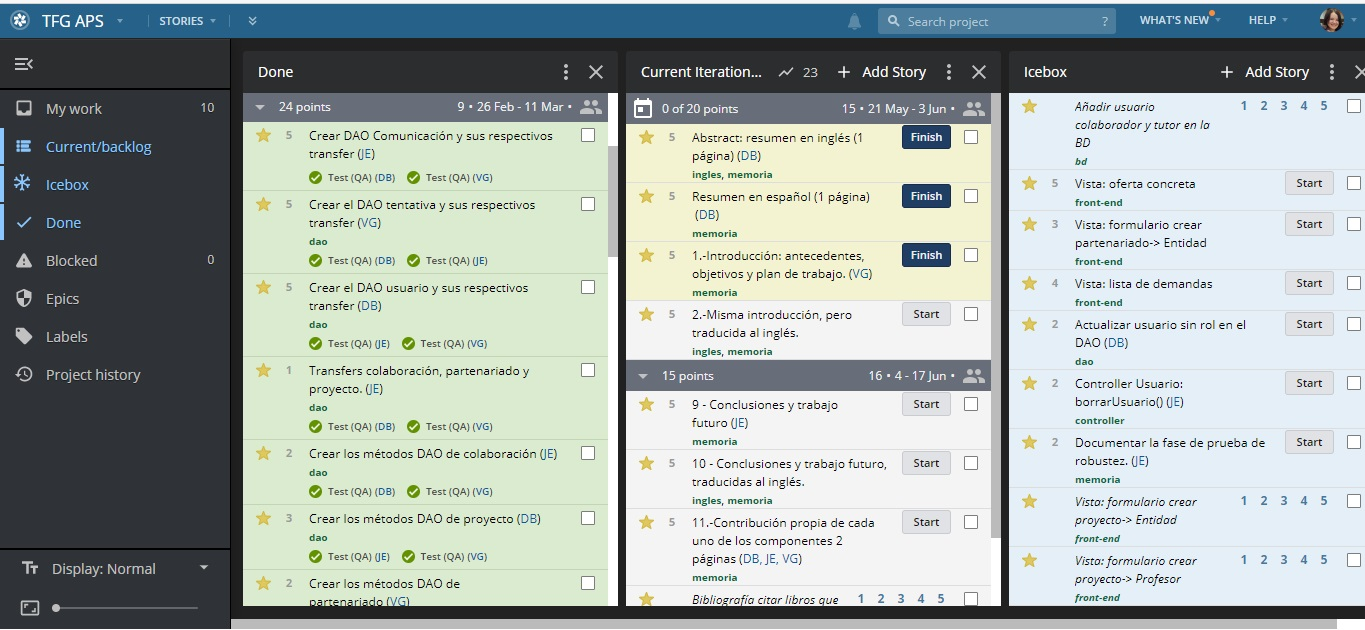
\includegraphics[scale=0.44]{pivotal2}
		\caption{PivotalTracker: tareas}
		\label{fig:pivotal2}
	\end{figure}
	\chapter{Contexto de la propuesta}\label{cap:contexto}
	\section{Introducción}
	El ApS es una propuesta educativa que combina aprendizaje y servicios a la comunidad. Los proyectos  ApS permiten a los alumnos aprender de una forma más práctica, aplicando sus conocimientos adquiridos en clase mediante la realización de tareas útiles para la comunidad. \\\\
	Además de dar a los estudiantes la oportunidad de aplicar sus conocimientos en un entorno real, el ApS les impulsa a comprender el funcionamiento de la sociedad y las responsabilidades sociales que estos tienen por formar parte de una sociedad.\\\\
	Todo proyecto ApS empieza por una iniciativa relacionada con una necesidad social real que implica la ejecución de un servicio para solventarla y tiene como objetivo el aprendizaje y la reflexión del alumno. Para saber más sobre el tema diríjase a la referencia \cite{rego2015aprendizaje}.
	\section{Elementos que intervienen en un proyecto ApS}
	En un proyecto ApS intervienen los siguientes elementos:
	\begin{itemize} 
		\item El \emph{alumno} es el individuo que aplica sus conocimientos teóricos en un entorno físico beneficiando a su comunidad. Además de adquirir habilidades prácticas relacionadas con su formación, es importante que se incite al alumno a reflexionar sobre sus actos y el impacto positivo que tienen estos sobre los demás. Esto permite al alumno adquirir compromiso social y desarrollar pensamiento ético, cultivando un ciudadano responsable capaz de mejorar la sociedad de la que forma parte.
		
		\item El \emph{socio comunitario} es una empresa pública o de tercer sector que colabora con la institución educativa para resolver un determinado problema social. El socio comunitario suele tener en mente un problema muy concreto, pero no lo suficientemente detallado para la creación de un proyecto educativo. Es por eso que es necesario el partenariado. Es importante que la universidad haga entender al socio comunitario que el ApS no es voluntariado. Por tanto, bajo ningún concepto se puede usar al alumno para la generación de beneficios propios de la empresa o la competencia desleal. El principal objetivo del ApS es formar al alumno introduciéndolo en un entorno real para que este establezca una relación entre lo aprendido en el aula con lo realizado en el proyecto ApS.
		
		\item El \emph{profesor} es el individuo que se encarga de guiar al alumno en todo el proceso del proyecto, evaluando sus tareas e incitando al alumno a la reflexión. Además de guiar al alumno en su formación y gestionar el proyecto, ofrece su formación y conocimientos al socio comunitario con la que se colaborará en el proyecto. El profesor se encarga de acordar y organizar los proyectos con el socio comunitario, estableciendo todos los requisitos necesarios para la correcta formación del alumno y el cumplimiento del socio comunitario con los principios del ApS.
		
		\item El \emph{partenariado} es una colaboración entre un profesor, o un equipo de profesores, y el socio comunitario. Partiendo de un problema social real y los conocimientos dispuestos por el profesor, el profesor y el socio comunitario determinan las características y particularidades del problema. Una vez definidos los términos y condiciones del futuro proyecto, el profesor abre el proyecto a otros profesores que quieran colaborar en las propuestas y posteriormente el proyecto se abre a los alumnos. Todo partenariado tiene un profesor responsable que pertenece a la universidad en la que se ha desplegado la aplicación.
		
		\item El \emph{proyecto} consiste en la ejecución de ciertas tareas realizadas por el alumno que están relacionadas con su formación. Estas tareas permiten al alumno establecer una relación entre lo aprendido en clase y el mundo real. Gracias a estas tareas o servicios, el alumno beneficia a su comunidad, otorgándole una satisfacción personal. El alumno es evaluado de forma continua por el equipo docente. Todo proyecto tiene un profesor responsable que pertenece a la universidad en la que se ha desplegado la aplicación.
	\end{itemize}
	\section{Motivación}\label{cap:cont-motidvacion}
	La motivación descrita a continuación ha sido extraída de nuestros directores los cuales conocen el histórico del proyecto:\\
	La experiencia de los profesores que han llevado a cabo, o intentado
	llevar a cabo, iniciativas de tipo ApS muestra
	que muchos proyectos potenciales no llegan a realizarse por la
	dificultad en casar la oferta con la demanda, es decir, cuadrar las
	necesidades didácticas, organizativas, etc. de la institución educativa
	que quiere prestar un servicio, con las necesidades y disponibilidad de
	la organización o comunidad que quiere recibir un servicio. El
	establecimiento de relaciones de partenariado en el ApS requiere tiempo
	y energía, siendo el análisis de compatibilidad entre la oferta y la
	demanda de servicios un aspecto clave. Los profesores con experiencia en
	iniciativas de tipo ApS, tanto de carácter local como en el contexto de
	proyectos de cooperación internacional para el desarrollo, se dieron
	cuenta hace tiempo de que un buen soporte informático podría ser de gran
	ayuda en la difícil tarea de casar la oferta y la demanda de ApS.
	Gracias a este soporte se facilitarían la identificación de potenciales
	partenariados, así como la colaboración entre el prestador y el receptor
	potenciales del servicio en la tarea de refinar una idea inicial y
	convertirla en una propuesta de proyecto realista que cumple las
	necesidades de las dos partes.\\\\
	
	Los programas de ApS, ya consolidados en el continente americano, tan
	solo recientemente empiezan a cobrar fuerza en las instituciones
	educativas europeas, y en particular en las españolas. Los primeros
	proyectos de ApS se iniciaron en nuestro país apenas hace 15 años.  El
	escaso valor académico concedido hasta ahora a la práctica del ApS fuera
	del ámbito de los estudios pedagógicos, ha sido motivo de que los
	intentos de desarrollar la aplicación informática descrita hayan surgido
	siempre en el contexto de PFC/TFG. El desarrollo de una tal aplicación
	requiere una alta dedicación y no tiene valor de investigación
	tecnológica, de modo que los profesores técnicamente cualificados no
	tienen disponibilidad para abordarlo.\\\\
	
	El PFC de Ingeniería Industrial de la
	\emph{Universidad Politécnica de Madrid} (UPM) \cite{ref1} fue el primer intento, según
	nuestro conocimiento, de desarrollar una aplicación para el soporte de
	la definición de PFC de cooperación (y del previo establecimiento de un
	partenariado Universidad-ONG) y dio como resultado una aplicación basada
	en el \emph{sistema de gestión de contenidos} (CMS) Plone. Sin embargo, su
	naturaleza de prototipo, junto con la falta de recursos humanos para su
	despliegue y administración, hizo que nunca llegara a utilizarse.
	Ángeles Manjarrés, profesora de la UNED, y Simon Pickin, uno de los directores del presente
	trabajo, retomaron la idea de \cite{ref1} en el TFG del grado en Informática de
	la UNED \cite{ref2}, en el que se desarrolló una aplicación web basada en el
	popular \emph{framework de gestión de contenidos} (CMF) Drupal. El prototipo
	desarrollado fue bastante básico e incompleto y tenía restricciones
	técnicas que limitaban su funcionalidad, pero constituyó un pequeño
	avance hacia el objetivo. Aunque el propósito del PFC \cite{ref1} y del TFG \cite{ref2}
	fue el soporte de la definición de PFC/TFG de cooperación, este objetivo
	puede verse como un caso particular del soporte de proyectos ApS y la
	plataforma informática necesaria es prácticamente idéntica en los dos casos.
	\\\\
	Se retomó la iniciativa de \cite{ref2} en el contexto de una colaboración entre
	la UCM y el grupo de investigación en innovación docente COETIC (“Grupo
	de Innovación Docente de la UNED para el Desarrollo de la Competencia
	Ética y Cívica y las metodologías basadas en la Comunidad en la
	educación superior”) con el TFG del grado en Educación Social de la UNED
	\cite{ref3}, centrado en la especificación de una aplicación para el soporte del
	ApS virtual, y los TFG del grado en Informática de la UNED \cite{ref4} y \cite{ref5},
	centrados en el desarrollo de tal aplicación, los dos últimos
	codirigidos por Ángeles Manjarrés y Simon Pickin. En \cite{ref4}, después de un
	intento fallido de continuar con el desarrollo en Drupal empezado en
	\cite{ref3}, debido a que Drupal resultó ser mucho más cerrado de lo esperado,
	se desarrolló una nueva aplicación desde cero basada en el stack MyEAN
	(\emph{MySQL-Express-Angular-Node}). Esta aplicación se describe brevemente en
	\cite{ref6}. En \cite{ref5}, se continuó el desarrollo de la aplicación de \cite{ref4} pero esta
	vez con el stack MEAN (\emph{MongoDB-Express-Angular-Node}); la substitución de
	MySQL por MongoDB no se debía a razones técnicas sino a razones de
	conveniencia y familiaridad del desarrollador. Aunque los títulos de \cite{ref4}
	y \cite{ref5} hacen referencia al ApS "Virtual", la aplicación desarrollada está
	pensada para dar servicio a toda la comunidad de ApS.
	
	
	\section{TFG de partida}
	El TFG de David Jiménez presentaba una base a partir de la cual hemos partido para desarrollar nuestra parte de este proyecto. Partiendo del TFG anterior que estaba desarrollado en Angular y Node.js, David Jiménez siguió desarrollando la aplicación hasta conseguir un prototipo de la futura aplicación.\\\\
	David Jiménez implementó las páginas de registro, \textit{login}, perfil, iniciativa y partenariado. También incluyó diferentes perfiles como el \textit{admin}, el socio comunitario, el profesor y el alumno.\\\\
	Por razones de comodidad y familiarización con la tecnología, en el TFG anterior se construyó la base de datos en MongoDB. Debido a que los datos de la aplicación son claramente estructurados y muy relacionados entre sí, no había razones suficientes para seguir desarrollando la aplicación sobre MongoDB, así que junto con nuestros directores decidimos cambiar la base de datos a SQL.\\\\
	Debido a las dificultades provocadas por la pandemia del COVID-19, las bases de la aplicación no quedaron del todo definidas en el TFG anterior y por esta razón hemos tenido que redefinirlas creando un modelo de dominio y de datos que representa todos los elementos del problema y cómo se relacionan entre sí. Diseñamos una base de datos nueva más compleja y rica en detalles que servirá como cimientos para nuestros sucesores, ya que esperamos que llegue el día en que esta plataforma sirva a usuarios reales, los cuales ayudaran a que la educación sea más eficaz y enriquecedora.
	
	\section{Estudio tecnológico}
	A continuación, se explicará qué tecnologías tienen el potencial para desarrollar este proyecto y cuáles hemos elegido finalmente. Las razones de las decisiones tomadas sobre el uso de estas tecnologías se detallan en la sección 4.
	\begin{enumerate} 
		\item Servidor web:
		\begin{itemize} 
			\item ExpressJS es un \textit{framework} basado en NodeJS que permite gestionar el servidor de una forma sencilla. Este \textit{framework} fue utilizado por David Jiménez en el TFG precursor y se ha mantenido.
		\end{itemize}
		\item \emph{Backend}: 
		\begin{itemize} 
			\item NodeJS es entorno basado en JavaScript muy popular. Este entorno fue usado en el anterior TFG y se ha mantenido.
		\end{itemize}
		\item \emph{Frontend}
		\begin{itemize} 
			\item Angular es un \textit{framework} utilizado en el \textit{frontend} del TFG anterior y se ha decidido mantener.
		\end{itemize}
		\item Base de datos: 
		\begin{itemize} 
			\item MongoDB es un sistema de base de datos no estructurado. Este sistema es el que se estaba usando en el proyecto.
			\item MySQL: es un sistema de base de datos relacional. Decidimos utilizar este sistema en nuestro TFG.
		\end{itemize}
		\item Software de control de versiones:
		\begin{itemize} 
			\item Git es el controlador de versiones más conocido y muy eficaz, así que desde el principio supimos que es el software que íbamos a usar. 
		\end{itemize}
		\item Repositorio: 
		\begin{itemize} 
			\item GitHub es un repositorio gratuito que permite almacenar todos los archivos relacionados con un proyecto y mantenerlos de forma colaborativa con otros usuarios. Se ha decidido utilizar GitHub por su integración con Git.
			\item Google Drive: es un contenedor gratuito que permite almacenar cualquier fichero y compartirlo con los demás. En un principio se estudió utilizar para guardar los \textit{Backups} pero se acabó descartando. Al final se ha utilizado para almacenar todo tipo de documentos relacionados con el TFG, excepto el código fuente de la aplicación.
		\end{itemize}
		\item Herramientas de organización: 
		\begin{itemize} 
			\item GitHub Projects es una herramienta que ofrece GitHub que permite crear una organización de proyecto tipo Kanban.
			\item Trello es una herramienta sencilla estilo Kanban para organizar los proyectos, pero tiene muchas limitaciones en su versión gratuita.
			\item PivotalTracker es una herramienta de gestión de proyectos basada en Scrum que permite crear \textit{Stories}, asignarles un peso en función de lo compleja que sea la \textit{Story} y ofrece analíticas que permiten analizar el progreso del proyecto. Hemos decidido utilizar esta herramienta para organizarnos porque es una herramienta completa.
		\end{itemize}
		\item Herramientas UML: 
		\begin{itemize} 
			\item Diagrams.net es una herramienta de diseño de diagramas \textit{online} la cual permite diseñar varios tipos de diagramas entre los cuales se encuentran diagramas de clases, de flujos, de entidades, etc.
			\item Modelio es una aplicación de escritorio que permite crear modelos UML complejos, indicando los atributos, los métodos y las relaciones que tienen los elementos entre sí. Debido a que es una herramienta completa y que es una herramienta que ya conociamos, la hemos elegido para la creación de nuestros modelos.
		\end{itemize}
		\item Herramientas para el diseño del modelo relacional de la base de datos: 
		\begin{itemize} 
			\item phpMyAdmin es una herramienta web que permite gestionar una base de datos SQL. Esta herramienta muestra un modelo relacional de la base de datos muy simple.
			\item MySQL Workbench es una herramienta de gestión de diseño de base de datos visual que permite crear modelos relacionales complejos. Esta es la aplicación que se ha decidido utilizar.
		\end{itemize}
		\item Herramientas para la redacción de la memoria:
		\begin{itemize} 
			\item Microsoft Word siendo una herramienta popular y muy conocida para la creación de documentos escritos, fue nuestra primera opción para la redacción de la memoria.
			\item LaTeX es una herramienta que permite crear documentos profesionales con resultados profesionales. Esta es la herramienta que se ha decidido utilizar.
		\end{itemize}
		\item Lenguaje para insertar datos en la BD:
		\begin{itemize} 
			\item Python se ha utilizado para insertar valores enumerados en la base de datos.
		\end{itemize}
	\end{enumerate}
	
	\chapter{Modelos de dominio, de datos y de relación}\label{cap:modelos}
	
	\section{Introducción}
	Al empezar con el proyecto, junto con nuestros directores, nos hemos dado cuenta de que la aplicación necesitaba ser definida de una forma más detallada. En TFGs anteriores se entendía que los profesores y las entidades definían los proyectos de la misma forma, pero esto no es así. Las entidades tienen un problema en mente que quieren resolver, pero no saben cómo adaptarlo a un proyecto estudiantil. Los profesores, por su parte, tienen una idea abstracta del problema que quieren resolver. Normalmente tienen ciertos conocimientos académicos los cuales quieren aplicar para mejorar el mundo, pero la necesidad social en cuestión no suele estar muy clara.\\\\
	En el TFG precedente se creó un elemento llamado \emph{Iniciativa} que almacenaba algunas de las características generales que comparten las propuestas del profesor y el socio comunitario. La \emph{Iniciativa} derivaba en un formulario que se les ofrecía a las entidades y a los profesores, pero las entidades y los profesores no plantean los problemas de la misma manera. Las entidades tienen una idea de proyecto clara pero no saben cómo orientarlo al mundo académico y los profesores tienen una idea de proyecto abstracta y lo plantean con el objetivo de encajar en un plan académico, es por esto que no es apropiado utilizar el mismo formulario para ambos.\\\\
	Para definir con precisión el funcionamiento correcto y completo de la aplicación, se ha creado un modelo de dominio y un modelo de datos.
	Estos modelos nos permitirán entender acertadamente el funcionamiento de la aplicación, pero lo que es más importante, permitirán transmitir dicho funcionamiento e idea general a otras personas que trabajarán en este proyecto después de nosotros.\\\\
	Gracias al modelo de dominio podemos entender qué elementos intervienen y cómo interactúan entre sí, además de las restricciones que se presentan en sus interacciones.\\\\
	Con el modelo de datos podemos conocer información detallada de cada elemento que interviene en la resolución del problema, así como los atributos que posee.\\\\
	Como se ha rediseñado la base de datos se ha decidido crear un modelo relacional que muestra todas las tablas de la nueva base de datos y sus relaciones. De esta manera, podemos representar sus especificaciones técnicas para comprender su estructura y funcionamiento. 
	
	\section{Modelo de dominio}
	El modelo de dominio es un mapa conceptual de la aplicación que permite a cualquier individuo entender su funcionamiento. El modelo de dominio de esta aplicación se puede observar en la Figura ~\ref{fig:dominio}.\\\\
	Si empezamos mirando nuestro modelo desde arriba podemos observar que hay una clase madre, llamada Usuario y de ella se ramifican otras cinco clases que representan los cinco grupos de usuarios que tiene la aplicación.\\
	\begin{itemize} 
		\item Los estudiantes se dividen en internos y externos. Los internos representan a aquellos estudiantes que pertenecen a la universidad donde está instalada la aplicación y los externos pertenecen a otras universidades.
		\item El grupo de usuarios promotor se divide en externos e internos por el mismo motivo que los estudiantes. 
		\begin{itemize} 
			\item El promotor externo representa al profesor externo, que es aquel profesor que no forma parte de la universidad donde está la aplicación, pero puede participar en un proyecto o partenariado evaluando y guiando a un estudiante externo. El colaborador, por otra parte, es un experto en algún tema en concreto que puede participar en un proyecto o partenariado ofreciendo sus conocimientos o habilidades. 
			\item El promotor interno puede ser un profesor de la universidad en la que se aloja la aplicación y también puede ser un tutor si pertenece a la UNED, donde existe este rol. El profesor interno puede crear las ofertas de servicio y es el responsable del partenariado y del proyecto.
		\end{itemize}
		\item El socio comunitario es aquella entidad que hace de socio para la creación del proyecto.
		\item El admin es el usuario administrador de la aplicación.
		\item La Oficina APS es un usuario responsable de todos los trámites relacionados con la gestión de los proyectos ApS. 
	\end{itemize}
	Todo proyecto tiene que definirse en el contexto de un partenariado y este partenariado se puede originar de varias maneras. \\
	Una de ellas es a partir de una oferta de servicio y una demanda de servicio. En este caso el partenariado puede surgir porque una de las dos partes decida aliarse con la otra buscándolo manualmente en la plataforma o porque el sistema de \textit{matching} sugiera la unión de ambas partes.
	Otra forma es mediante la creación de lo que llamamos partenariados ``monoparentales'', es decir, partenariados
	creados cuando un socio comunitario acepta una oferta creada por un
	profesor sin haber creado previamente una demanda, o cuando un profesor
	respalda una demanda creada por un socio comunitario sin haber creado
	previamente una oferta. En estos casos, la correspondiente oferta (resp.
	demanda) se creará en el momento de aceptar (resp. respaldar) la oferta
	(resp. la demanda) y se utilizará un atributo de la oferta y de la
	demanda para almacenar la naturaleza ``monoparental'' del partenariado.\\\\
	En general una demanda de servicio es creada por un socio comunitario, pero puede llegar a crearse gracias a un estudiante, el cual previamente ha tenido que crear una iniciativa. Una iniciativa es una propuesta de proyecto de un estudiante, la cual es acogida por un socio comunitario despues de haber sido aprobada por la oficina ApS. Cuando el socio comunitario acoge dicha iniciativa, esta se convierte en una demanda de servicio.\\
	Debido a que los proyectos definidos por los profesores y los definidos por las entidades comparten ciertas características, podemos ver en el diagrama que ambos cuelgan de un elemento padre llamado \textbf{Anuncio de servicio} que posee las características comunes de ambos.
	Lo mismo ocurre con \textbf{partenariado} y \textbf{proyecto} que cuelgan de \textbf{Colaboración Uni-Soc}.\\
	Queremos destacar que los atributos de \textbf{Necesidad social} y \textbf{Area de implementación}, tan importantes para emparejar ofertas y demandas, han sido obtenidos de la página web \url{www.eoslhe.eu/resources/}
	Los partenariados y los proyectos presentan ciertas restricciones relacionadas con la participación de alumnos y promotores externos.\\\\
	En los proyectos solo pueden participar estudiantes externos si el responsable del proyecto acepta estudiantes externos. 
	Los profesores externos solo pueden participar en aquellos partenariados y proyectos que los acepten. Además, en el caso de un proyecto, un participante solo puede tener el
	perfil de profesor externo si también participan alumnos externos de su
	universidad, cuya participación tendrá que evaluar; en otro caso, tendrá
	el perfil de colaborador, independientemente del tipo de puesto que
	ocupa en su universidad.\\\\
	\begin{landscape}
		\begin{figure}[p]
			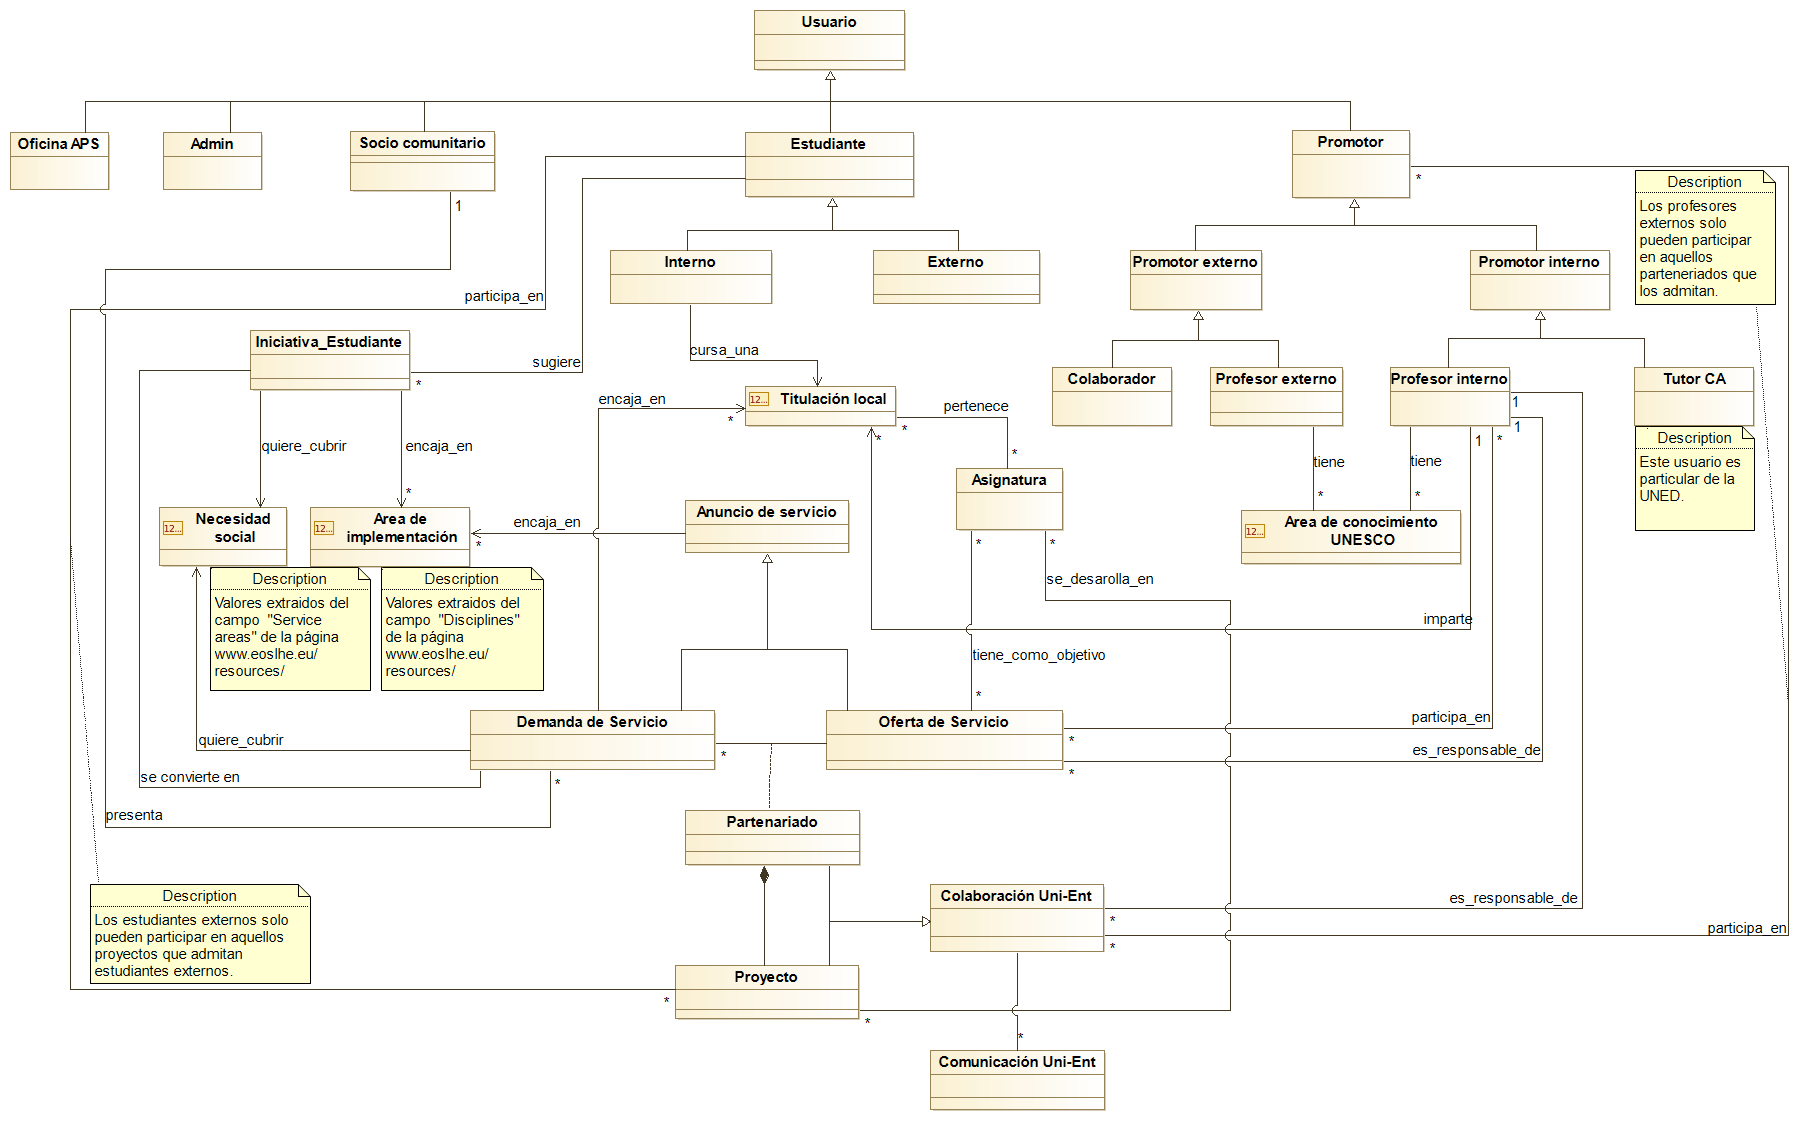
\includegraphics[scale=0.4]{mdominio}
			\caption{Modelo de dominio}
			\label{fig:dominio}
		\end{figure}
	\end{landscape}
	\begin{landscape}
		\begin{figure}[p]
			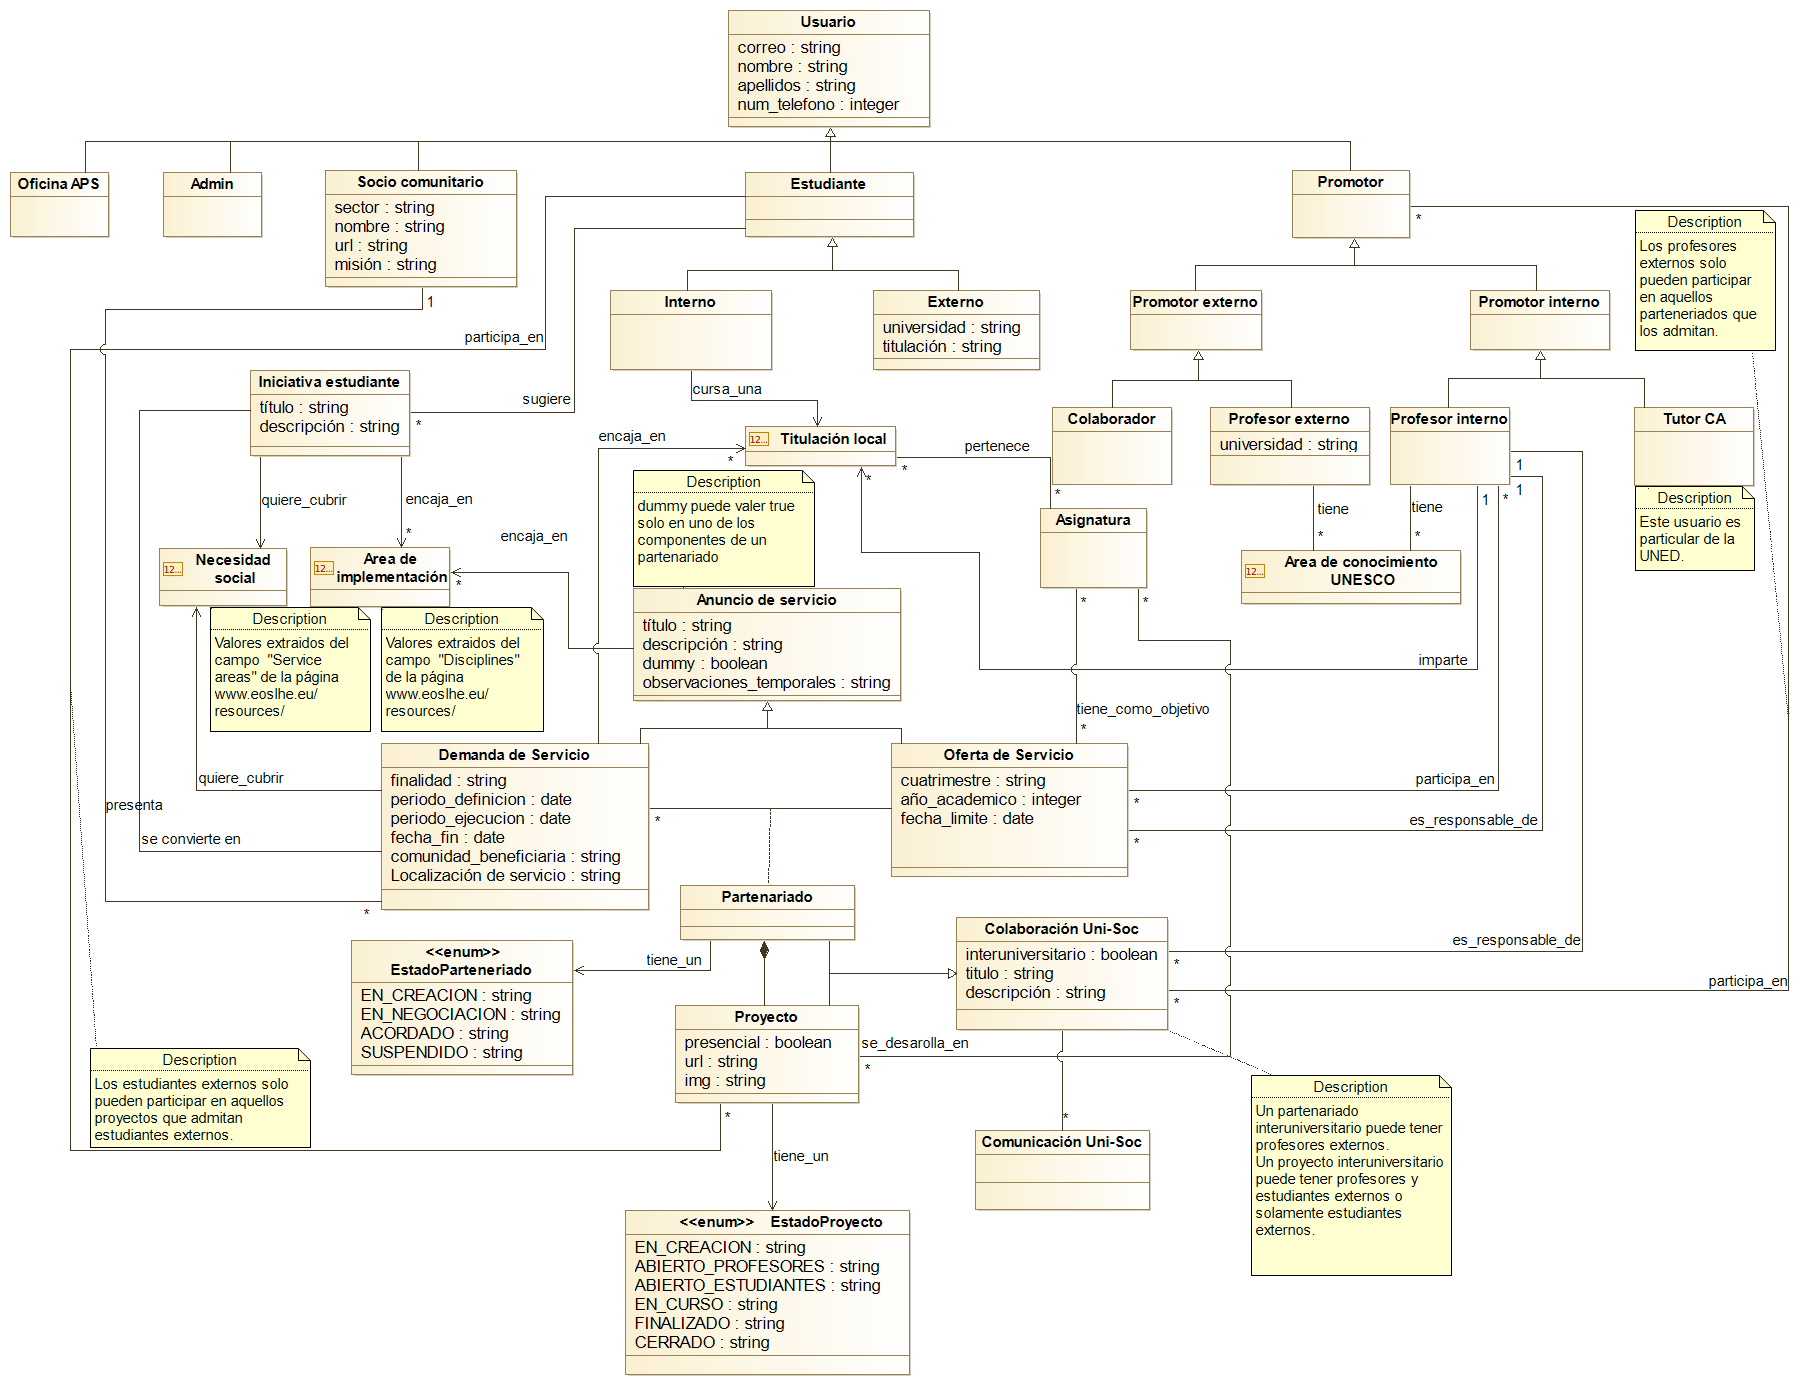
\includegraphics[scale=0.35]{mdatos}
			\caption{Modelo de datos}
			\label{fig:datos}
		\end{figure}
	\end{landscape}
	
	\section{Modelo de datos}
	El modelo de datos describe con más precisión el dominio de la aplicación.
	Además de algunos atributos importantes como el interuniversitario, que indica si el partenariado o el proyecto está abierto a externos, podemos observar los estados que pueden tener el partenariado y el proyecto, representados por dos enumerados. En particular podemos ver que el partenariado puede encontrarse en estados \texttt{EN\_CREACION}, \texttt{EN\_NEGOCIACION}, \texttt{ACORDADO} y \texttt{SUSPENDIDO}. El modelo de datos se puede observar en la Figura ~\ref{fig:datos}.\\
	\begin{itemize} 
		\item El partenariado se crea en el estado \textit{EN\_CREACION} o bien cuando un
		profesor interno respalda a una demanda presentada previamente por un
		socio comunitario o acepta un \textit{match} de una oferta y demanda propuesto
		por la aplicación, o bien cuando un socio comunitario acepta una oferta
		presentada previamente por un profesor interno. Cuando la otra parte da su asentimiento a la creación del partenariado, su estado pasa a ser \textit{EN\_NEGOCIACION}. Cuando el profesor y el socio comunitario terminan de establecer los términos y condiciones del partenariado y ambos están de acuerdo con dichos terminos, el partenariado pasá a estar \texttt{ACORDADO}. Si ocurre cualquier discrepancia durante la fase de \texttt{EN\_CREACION}, \texttt{EN\_NEGOCIACION} o \texttt{ACORDADO} el partenariado puede pasar al estado de \texttt{SUSPENDIDO}.
		\item El proyecto toma los estados \texttt{EN\_CREACION}, \texttt{ABIERTO\_PROFESORES}, \texttt{ABIERTO\_ESTUDIANTES}, \texttt{EN\_CURSO}, \texttt{FINALIZADO} y \texttt{CERRADO}.
		El profesor interno responsable de un partenariado en estado \texttt{ACORDADO}  puede pedir que se cree un proyecto derivado de este partenariado. El
		estado inicial de un proyecto es \texttt{EN\_CREACIÓN}. Cuando el socio
		comunitario da su asentimiento a la creación del proyecto, su estado
		pasa a ser \texttt{ABIERTO\_PROFESORES}. Una vez terminada la definición del proyecto se abre a los alumnos y es allí cuando el proyecto pasa al estado de \texttt{ABIERTO\_ESTUDIANTES}. Si el proyecto finaliza correctamente, pasará al estado de \texttt{FINALIZADO}. Si sucede cualquier imprevisto durante las 4 fases anteriores el proyecto puede pasar al estado \texttt{CERRADO}.
	\end{itemize} 
	
	\section{Modelo relacional}
	Debido a la complejidad de la nueva base de datos compuesta por 46 tablas relacionales, se ha decidido crear un diagrama que sirva como mapa en la gestión de la base de datos. Este modelo relacional se divide en cuatro secciones claramente diferenciadas.
	\begin{itemize} 
		\item La sección de los usuarios que contiene tablas relacionadas con información de los usuarios. La sección del \textbf{Anuncio de servicio} que contiene todas las tablas que representan información de las ofertas de servicio, las demandas de servicio y las iniciativas.
		\item La sección de \textbf{Colaboración} contiene la información relacionada con los partenariados y los proyectos.
		\item La sección de Comunicación que contiene las tablas de \textit{mail}, mensaje, \textit{upload} y \textit{newsletter}, estas fueron creadas por David Jiménez en los documentos de MongoDB cuya estructura se ha mantenido intacta.
		En la Figura \ref{fig:relacional} se puede observar el modelo relacional y sus cuatro secciones separadas por colores.
	\end{itemize}
	\begin{landscape}
		\begin{figure}[p]
			\centering
			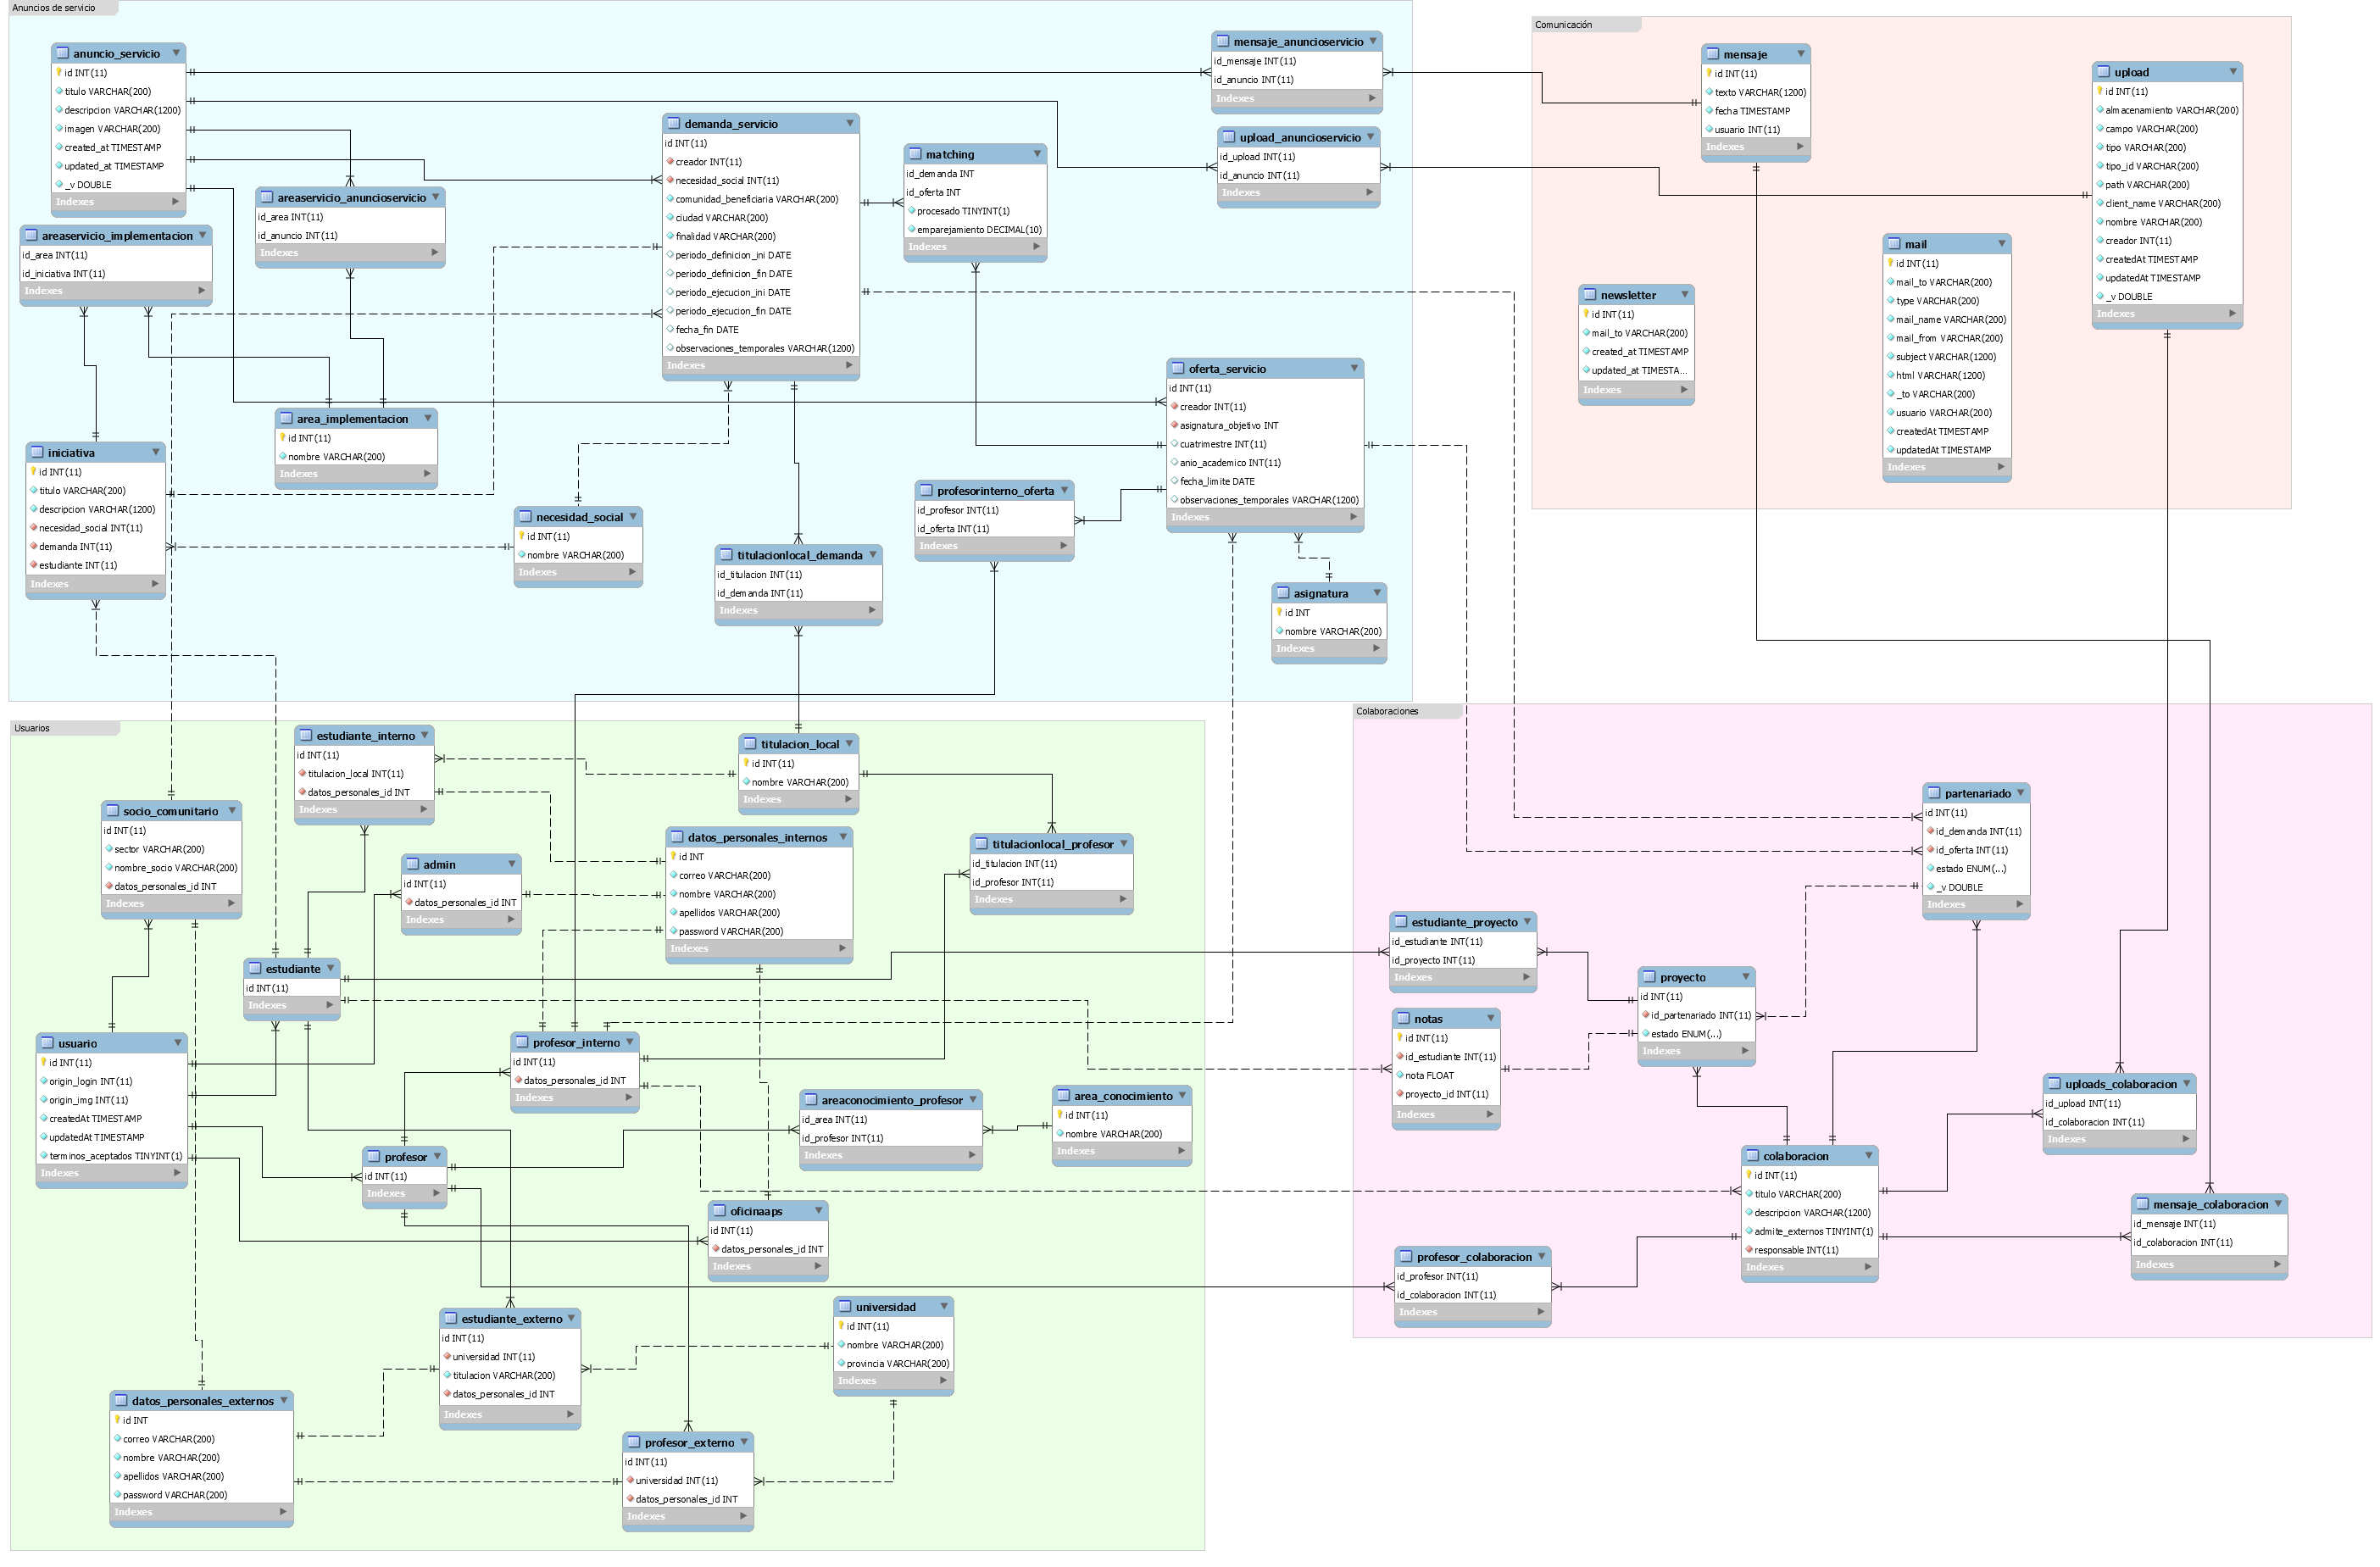
\includegraphics[scale=0.25]{er}
			\caption{Diagrama de entidad-relación}
			\label{fig:relacional}
		\end{figure}
	\end{landscape}
	
	\subsection{Separación de datos}
	Una cosa importante para destacar es que, en un entorno real, la aplicación cogería parte de los datos de los usuarios de la base de datos de la universidad en la que se despliegue la aplicación. Es por esto por lo que los datos de los usuarios se han separado en dos grupos; internos y externos. Los usuarios internos son aquellos que pertenecen a la universidad en la que se ha desplegado la aplicación y por ello utilizan SSO (Single Sign-On) de la universidad para acceder a la aplicación. Esta separación de datos se ha hecho con el propósito de facilitar la transición entre la base de datos del prototipo y la base de datos de la aplicación real.\\
	En concreto, los datos que son afectados por esta separación son el correo electrónico, el nombre, los apellidos y la contraseña que deberían alojarse en la base de datos de la universidad.
	\subsection{Usuarios}
	Esta sección es la más compleja debido a la separación que hay que realizar de los usuarios externos e internos. Ver Figura \ref{fig:usuarios}.\\
	Un usuario interno es aquel profesor, tutor, estudiante, administrador o representante de la oficina ApS que forma parte de la universidad en la que se despliega la plataforma y por tanto tiene sus datos personales dentro de ella. Debido a que, en un despliegue real tendrían parte de los datos que necesitamos para la aplicación en el sistema interno de la universidad, hay que tratarlos de manera diferente a los usuarios externos, que son aquellos que no pertenecen a la universidad. Los colaboradores y directores que aquí mencionamos se pueden ver representados en el modelo de datos y de dominio, pero no se observan aquí porque no nos dio tiempo a integrarlos en la base de datos.\\\\
	Debido a esta separación, todos los usuarios comparten una tabla común, llamada usuario, que contiene datos exclusivos de la cuenta de la plataforma. Después tenemos tablas que contienen datos particulares de cada tipo de usuario. Estas son las tablas del \textit{socio comunitario}, estudiante interno, estudiante externo, \textit{admin}, profesor interno, profesor externo y oficina ApS.\\
	Cada uno de estos usuarios poseen una tabla que almacena sus datos personales, haciendo diferenciación entre internos y externos. La tabla de datos\_personales\_internos es una tabla creada para la simulación de la aplicación. Una vez la aplicación sea desplegada en un entorno real, esta tabla será eliminada y los datos personales se obtendrán haciendo consultas a la base de datos de la universidad.\\
	Por otra parte, podemos observar tablas secundarias que representan características de los usuarios como por ejemplo, la universidad del profesor y estudiante interno, las áreas de conocimiento UNESCO de los profesores y las titulaciones que imparten los profesores o cursan los alumnos.
	\begin{landscape}
		\begin{figure}[p]
			\centering
			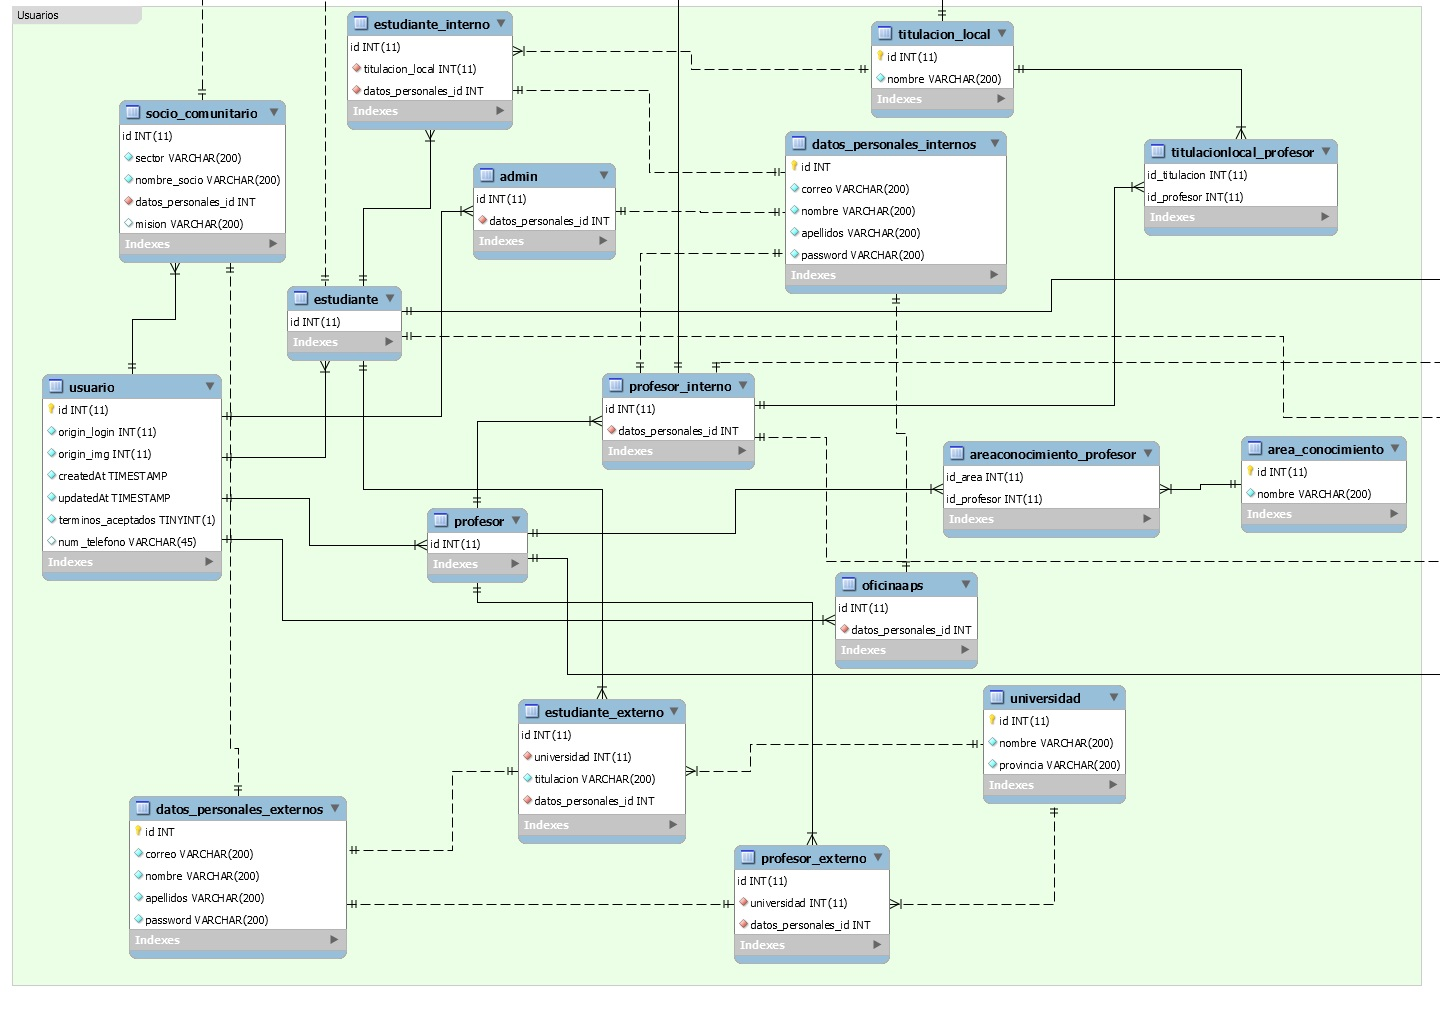
\includegraphics[scale=0.6]{usuarios}
			\caption{Diagrama de entidad-relación - Usuarios}
			\label{fig:usuarios}
		\end{figure}
	\end{landscape}
	
	\subsection{Anuncios de servicio}
	En este conjunto de tablas podemos encontrar las pertenecientes a la demanda de servicio, la oferta de servicio y la iniciativa. Ver Figura \ref{fig:anuncios}.
	\begin{itemize} 
		\item La iniciativa es una propuesta de proyecto realizada por un estudiante. Esta propuesta debe ser validada por la oficina ApS, que estudiará si la propuesta es viable para ser adoptada por un socio comunitario. Una vez validada la iniciativa, puede ser adoptada por un socio comunitario que desee realizar el proyecto.
		\item La demanda de servicio es creada por un socio comunitario y define una necesidad especifica que quiere cubrir. Esta necesidad social es representada por los elementos de un enumerado alojado en la tabla de necesidad\_social. Esta demanda
		\item La oferta de servicio es creada por un profesor interno y suele tener menos detalles que la demanda porque suele ser una propuesta más genérica.\\
		Cuando una oferta y una demanda son procesadas por el sistema de \textit{matching} se crea una entrada en la tabla \textit{matching} almacenando los \textit{ids} de ambos elementos y el porcentaje de emparejamiento que tienen.\\
		Tanto demanda de servicio como oferta de servicio están conectadas a mensajes y \textit{uploads} porque estos permiten la comunicación con las personas interesadas en las propuestas.
	\end{itemize}
	\begin{landscape}
		\begin{figure}[p]
			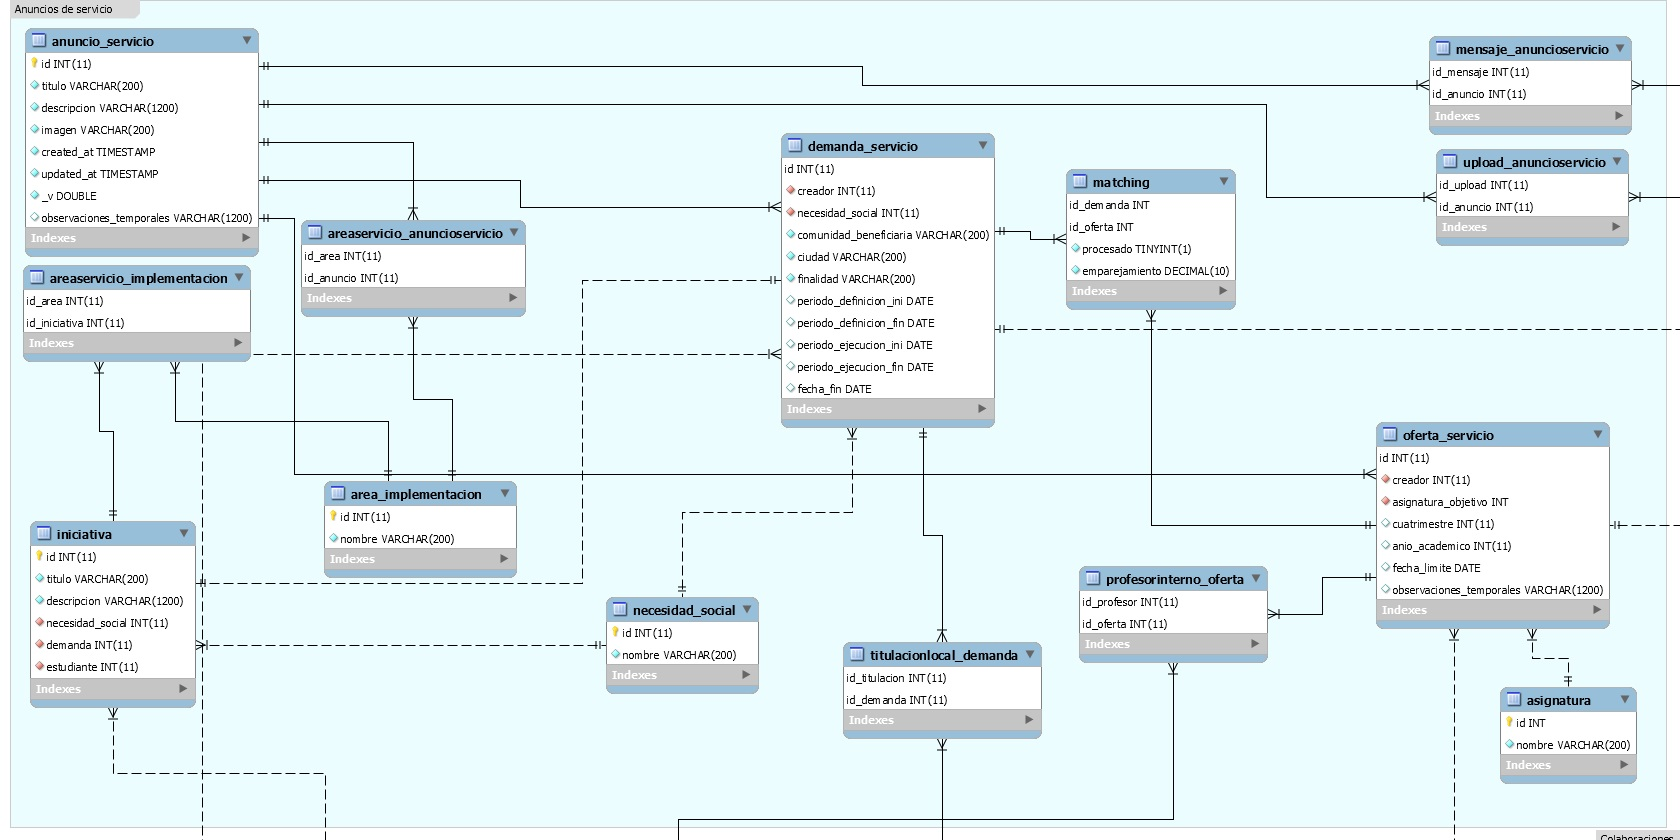
\includegraphics[scale=0.54]{anuncios}
			\caption{Diagrama de entidad-relación - Anuncios de servicio}
			\label{fig:anuncios}
		\end{figure}
	\end{landscape}
	
	\subsection{Colaboración}
	El partenariado es el segundo paso en la creación de un proyecto. Esta tabla contiene los \textit{ids} de la demanda y la oferta que la componen.\\
	Un proyecto ApS no puede existir sin un partenariado previo y es por eso por lo que tiene un identificador del partenariado a partir del cual se creó. El proyecto posee estudiantes y por ello tiene una conexión con los mismos.\\
	Tanto proyecto como partenariado necesitan un sistema de comunicación y es por eso por lo que tienen tablas intermedias que los conectan a mensaje y \textit{uploads}. Ver Figura \ref{fig:colaboracion}.
	\begin{landscape}
		\begin{figure}[p]
			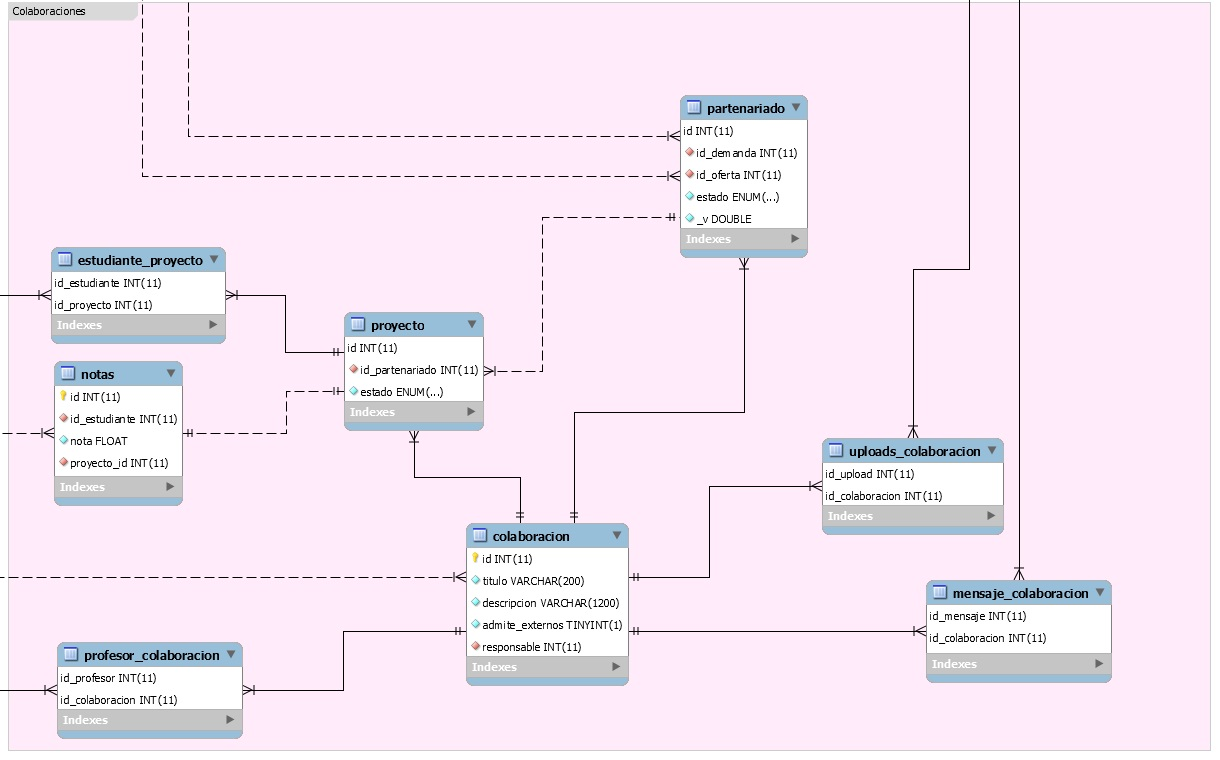
\includegraphics[scale=0.6]{colaboracion}
			\caption{Diagrama de entidad-relación - Colaboración}
			\label{fig:colaboracion}
		\end{figure}
	\end{landscape}
	\subsection{Comunicación}
	Las funcionalidades de estas tablas no han sido del todo definidas, ya que en un principio se pensó que podrían comunicar al equipo docente con los socios comunitarios en los partenariados y los proyectos, pero también se podrían usar para la comunicación con los creadores de las ofertas y las demandas. Debido a que el funcionamiento no ha sido estudiado aun y que no hemos trabajado con estas tablas en nuestro TFG, se ha mantenido la misma estructura que había definido David Jiménez en sus colecciones de MongoDB adaptándola al modelo relacional. Ver Figura \ref{fig:comunicacion}. 
	\begin{itemize} 
		\item La tabla de mensajes conecta con las ofertas de servicio, las demandas de servicio, los partenariados y los proyectos porque todos estos necesitan de los mensajes para poder comunicarse.
		\item La tabla \textit{upload} almacena la información de los ficheros e imágenes subidos tanto en ofertas de servicio, como demandas de servicio, como partenariados y proyectos.
		\item La tabla \textit{mail} y \textit{newsletter} no han sido conectadas con ninguna otra tabla porque no se han tenido en cuenta para el desarrollo de este TFG, pero representan los correos electrónicos internos de la aplicación y las noticias periódicas enviadas a los usuarios.
	\end{itemize}
	\begin{figure}[t]
		\centering
		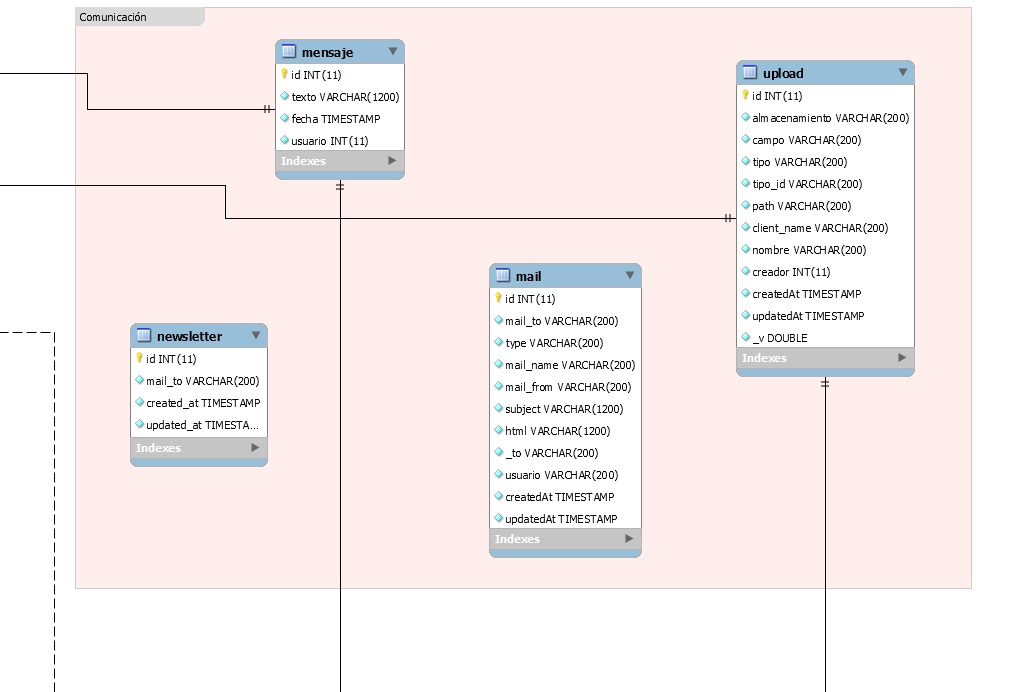
\includegraphics[scale=0.6]{comunicacion}
		\caption{Diagrama de entidad-relación - Comunicación}
		\label{fig:comunicacion}
	\end{figure}
	
	\chapter{Contribución}
	A continuación, se detallan las contribuciones de cada uno de los componentes del grupo ordenados por orden alfabético.
	\section{Daniela-Nicoleta Boldureanu}
	\section{Victoria Gnatiuk Romaniuk}
	La primera fase era una fase de investigación así que en esta fase todos hemos investigado y no hay ninguna tarea individual que destacar.\\\\
	En la segunda fase del proyecto Victoria se ha encargado de arreglar algunos \textit{bugs} del trabajo anterior. Los \textit{bugs} eran fáciles de arreglar, uno de ellos era que en el formulario de registro en los campos correo, nombre y apellidos se pedía al usuario que introdujera lo mismo, que era el nombre. Otra cosa que no era un \textit{bug} si no más bien una mejora, era que al editar el perfil de usuario se pedía volver a aceptar las condiciones de uso, cosa que veíamos innecesaria.\\\\
	En la tercera fase del TFG Victoria se ha encargado de continuar el modelo de dominio y el modelo de datos usando Modelio. En paralelo ha creado las tablas \textbf{profesor\_externo, iniciativa, anuncio\_servicio, demanda\_servicio, oferta\_servicio, partenariado, proyecto, colaboracion, newsletter y entidad\_demanda} en la base de datos. También ha creado las tablas que alojan los valores de los enumerados como la tabla \textbf{area\_implemetación, necesidad\_social, area\_conocimiento, universidad, titulacion\_local} y las tablas intermedias que permiten conectar las tablas de los enumerados con las tablas que las referencian. Con crear las tablas nos referimos a crear la estructura, definiendo los nombres de los campos y los tipos de datos, y creando restricciones entre las tablas.\\
	Una vez todas las tablas fueron creadas usando MySql Workbench 8.0 CE, Victoria creó el modelo relacional a partir del fichero SQL. Después hubo que distribuir todas las tablas en los cuatro grupos explicados en el capítulo \ref{fig:relacional} para que todas las tablas fueran debidamente visibles.\\\\
	En la fase cuatro Victoria se ha encargado de desarrollar el DAO llamado \textit{Tentativa} que implementa el acceso a la base de datos del grupo de tablas llamado \textit{Anuncios de servicio} que se puede ver en la Figura \ref{fig:anuncios}. La creación de este DAO ha supuesto la necesidad de la creación de tres \textit{transfers} que alojan los datos del elemento Anuncio de servicio, Demanda de servicio y Oferta de servicio. Los daos han sido implementados usando Knex.js, una librería que facilita las consultas a la base de datos. En el DAO \textit{Tentativa} se crearon las funciones CRUD, 3 de cada tipo concretamente. Dos de ellas eran las de la oferta y la demanda y la tercera, la cual siempre se llama desde las otras dos, es la del anuncio de servicio. También se creo el método para obtener todas las iniciativas, todas las demandas y todas las ofertas. Además de estos métodos, se han creado otros necesarios para la creación de los formularios de crear oferta y demanda. \\
	Después de finalizar la implementación del DAO \textit{Tentativa} Victoria desarrolló en los métodos CRUD del elemento \textit{Partenariado} perteneciente al DAO \textit{Colaboración}. Este DAO implementa las tablas pertenecientes al grupo \textit{Colaboración} que se puede ver en esta Figura \ref{fig:colaboracion}.
	Después Victoria implementó en el DAO \textit{Usuarios} dos métodos para obtener cualquier tipo de usuario con el id y con el correo del usuario. Estos métodos eran necesarios para la adaptación de la página de registro y \textit{login} al nuevo sistema. Junto con Jesús, Victoria adaptó el \textit{login} al nuevo sistema.\\\\
	En la fase cinco Victoria se ha encargado de crear el método que determina la similitud que tiene los campos \textbf{area\_implementación}, perteneciente a la \textit{Oferta de servicio} y \textbf{area\_conocimiento}, perteneciente a la \textit{Demanda de servicio}. Para esto se ha tenido que crear un Excel donde los valores de los enumerados de \textbf{area\_implementación} se han colocado en la primera fila y los valores de los enumerados de  \textbf{area\_conocimiento} se han colocado en la primera columna. Posteriormente se han colocado \textit{X} para marcar la similitud entre los valores, está similitud ha sido determinada por Victoria. Después de crear el Excel se ha creado un \textit{script} con Python que leía este Excel e insertaba los emparejamientos en una tabla de la base de datos, de la cual se leerá posteriormente para determinar si estos dos enumerados pueden ser emparejados. A continuación, se creó el método que compraba estos enumerados. Se hizo este mismo proceso para determinar el emparejamiento entre \textbf{area\_implementación}, perteneciente a la \textit{Oferta de servicio} y \textbf{titulacion\_local}, perteneciente a la \textit{Demanda de servicio}.\\
	Además de estos métodos para determinar el \textit{matching}, Victoria implemento otros dos. Uno de ellos determinaba si las dos \textbf{areas\_implementación}, pertenecientes a Oferta de servicio y Demanda de servicio coinciden. El segundo método determinaba si coincidían las titulaciones de la \textit{Demanda de servicio} y las titulaciones que imparte el profesor que ha creado la \textit{Oferta de servicio}.\\\\
	En la fase cinco Victoria se ha encargado de implementar el formulario para crear la oferta de servicio y también ha desarrollado la parte \textit{back-end} del formulario para crear el partenariado por parte del profesor y por parte del socio comunitario.
	Conjuntamente con todo esto Victoria ha ido actualizando los modelos de dominio y de datos a medida que iban sufriendo cambios a causa de los cambios sugeridos por los directores del TFG. También ha mantenido actualizado el diagrama relacional a medida que la base de datos iba sufriendo cambios.
	\section{Jesús Sánchez Granado}
	\bibliography{referencias}
=======
\end{titlepage}

%Indice

\tableofcontents
\newpage
\listoffigures

\chapter{Tecnologías utilizadas}
A continuación, se hablará sobre las tecnologías utilizadas explicando brevemente que son y los motivos por los que han sido seleccionadas.

\section{Node.js} 
Node.js \cite{node} es un entorno de ejecución asíncrono dirigido por eventos. Funciona a base de promesas, es decir, funciones que devolverán un resultado en algún momento del futuro. Las promesas se pueden encadenar una tras otra, recibiendo cada una el resultado de la anterior.\\\\
Esta forma de conseguir concurrencia es distinta a la manera más común que es utilizando cierres de exclusión mutua o candados. Los candados funcionan de la siguiente manera: si durante la ejecución de un programa concurrente un elemento es compartido por varios hilos, el resultado dependerá de las operaciones y el orden en que se lleven a cabo las mismas en dicho elemento. Para evitar que dos hilos accedan de manera simultánea a un mismo recurso, hay que ``bloquear'' ese recurso utilizando candados, llegando a la situación conocida como exclusion mutua ,pero cuando hay varios procesos concurrentes puede darse la situación de que el proceso A esté esperando a que el proceso B libere un recurso, y al mismo tiempo B espera que A libere un recurso. Esta situación se conoce como \emph{deadlock} o interbloqueo y es un bloqueo infinito.\\\\
Node.js no utiliza cierres de exclusión mutua o candados, por lo que es imposible que el programa alcance el estado de \emph{deadlock}, lo que lo hace bastante adecuado para desarrollar sistemas escalables.\\
Otro motivo para continuar con esta tecnología es que Daniela ya tenía conocimiento previo de este entorno y es una tecnología que venía impuesta por el proyecto.

\section{Angular}
Angular \cite{angular} es un \emph{framework} para la construcción de aplicaciones de página única (SPA a partir de ahora) que utiliza HTML y Typescript. Angular sigue el patrón modelo-vista-controlador, el cual consiste en separar la aplicación en tres partes:
\begin{itemize}
	\item Modelo: Es la piedra angular del patrón, se encarga de manejar los datos y la lógica de la aplicación.
	\item Vista: Es la parte que se le muestra al usuario.
	\item Controlador: Es la parte que se encarga de comunicar a la vista y al modelo. El controlador recibe los eventos de interacción del usuario a través de la vista y se los pasa al modelo, el cual hace las operaciones necesarias y devuelve los resultados al controlador, quien se los pasa a la vista para mostrárselos al usuario.
\end{itemize}


El uso de Angular venía impuesto por el trabajo realizado con anterioridad y, aunque es una tecnología con la que ningún miembro del equipo estaba familiarizado, es cierto que el diseño de aplicación de página única hace mucho más liviana la ejecución de la aplicación por parte del usuario, al no tener unos tiempos de espera tan grandes como los que tendría al cargar de nuevo cada página. Esto hace de Angular una buena elección para un trabajo de esta índole.

\section{GitKraken}
Gitkraken es un cliente de Git con interfaz de usuario la cual se puede conectar a distintas plataformas de Git, haciendo de intermediario entre el usuario y el repositorio de Git, el cual en este caso está alojado en Github. Hemos escogido esta interfaz para nuestro control de versiones porque permite trabajar desde Windows sin necesidad de conocer los comandos de Git. A diferencia de otros clientes de Git, tiene una representación gráfica muy intuitiva que permite ver la distribución de las ramas, los \emph{commits} y su evolución, como se puede observar en la Figura \ref{Figura 1}, y además permite resolver los conflictos generados al mezclar las distintas ramas de desarrollo dentro de la propia aplicación de una manera bastante sencilla. Esto, sumado a la experiencia previa de Victoria con la aplicación, ha hecho que sea seleccionada como herramienta de control de versiones.
\begin{figure}
	\centering
	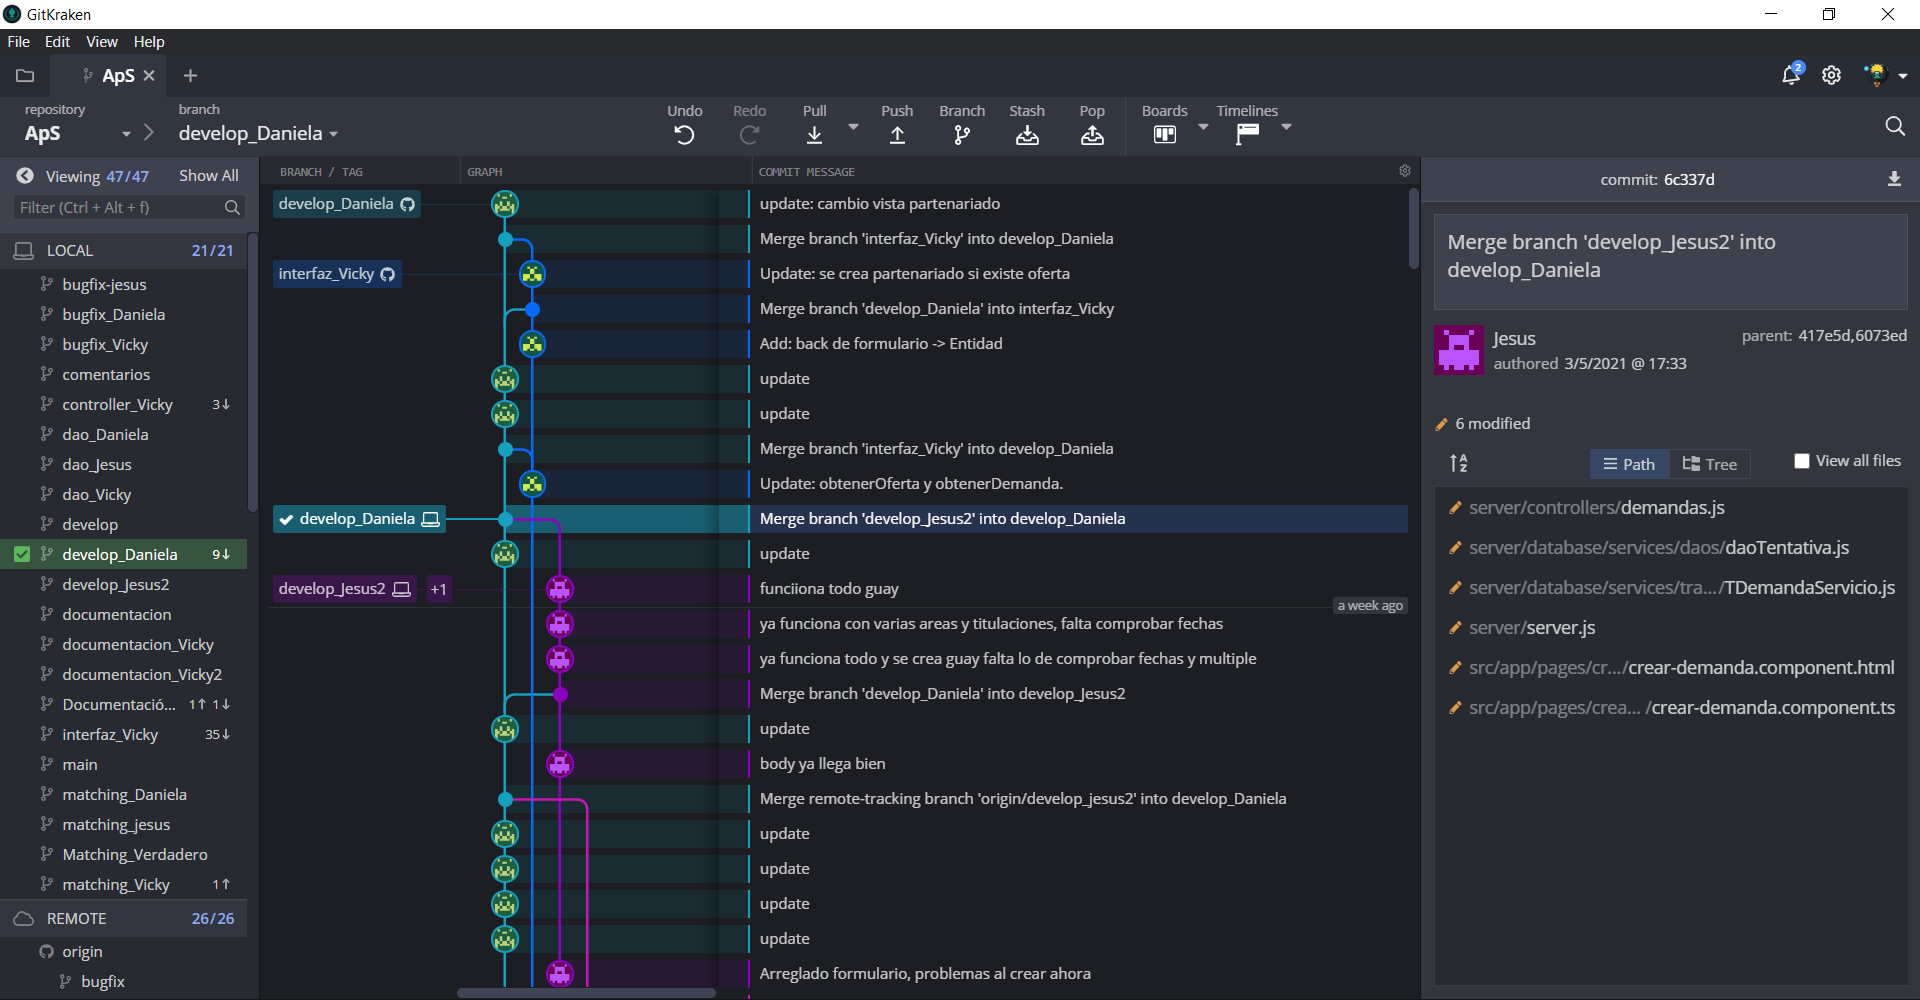
\includegraphics[scale=0.4]{gitkraken}
	\caption{GitKraken: Información de una rama de desarrollo}
	\label{Figura 1}
\end{figure}

\section{Pivotal tracker}
Pivotal tracker es una herramienta de \emph{product planning} y administración de tareas diseñada para equipos de desarrollo que siguen metodologías de diseño ágiles.
Esta herramienta permite crear historias de usuario y asignarles una puntuación del 1 al 5 indicando su dificultad y/o tiempo invertido en dichas tareas. Además, permite cambiar el estado de las tareas (empezado, finalizado, en revisión, etc.) y cualquier cambio en el estado de dichas tareas se informa por correo de manera automática a quien esté involucrado en ella.
También permite ver las tareas completadas y rechazadas y generar gráficos indicando el esfuerzo realizado, como el que podemos ver en la figura \ref{Figura 2}. Esta tecnología fue sugerida por Victoria y nos ha facilitado mucho tanto la organización como el seguimiento de nuestros avances.

\begin{figure}
	\centering
	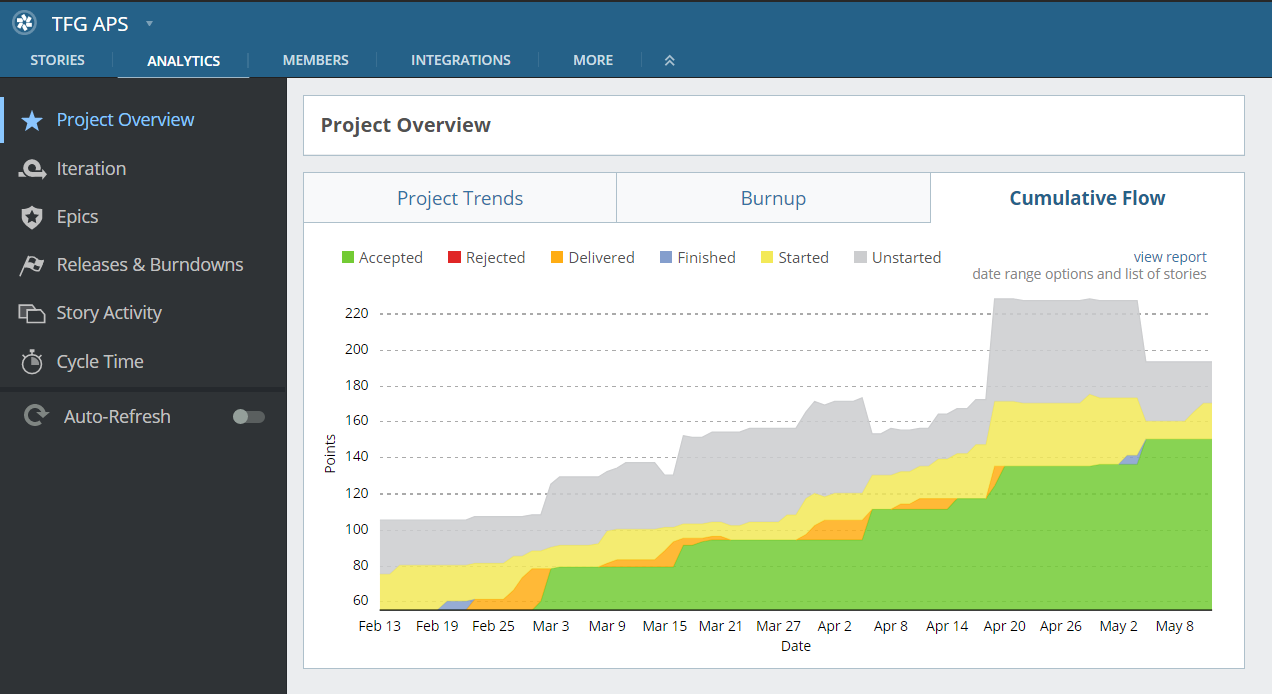
\includegraphics[scale=0.6]{pivotal}
	\caption{Pivotal tracker: Estadísticas de historias}
	\label{Figura 2}
\end{figure}

\section{\LaTeX}
\LaTeX es un lenguaje de creación de documentos escritos utilizado comúnmente en el mundo académico, que es una de las principales razones por la que lo hemos escogido para redactar nuestra memoria, a pesar de que ningún integrante del grupo tuviera experiencia previa con ello. A diferencia de otros procesadores de texto, como Microsoft Word o LibreOffice Writer, se escribe el texto plano y se formatea dicho texto con etiquetas. 

\section{MySQL}
Aunque nuestro proyecto continúa el trabajo realizado por David Jiménez del Rey, el cual ya contaba con un sistema gestor de bases de datos, dicho sistema era MongoDB. Como los datos que se iban a manejar en la aplicación eran en su mayoría relacionales se tomó la decisión de utilizar MySQL para la base de datos. Dado que todos los componentes del grupo tenían experiencia previa en bases de datos SQL fue un cambio bien recibido.

\section{Modelio}	
Modelio es un entorno de modelado \emph{open-source} el cual permite trabajar con un amplio rango de modelos y diagramas. Dado que ya se contaba con experiencia previa en esta herramienta por parte de todos los miembros del equipo, se ha escogido para realizar los modelos de datos necesarios para la aplicación.

\section{MySQL Workbench}
MySQL Workbench es una herramienta para diseño, desarrollo y administración de bases de datos relacionales. 
Cuenta con funcionalidades de validación de esquemas y modelos y promueve las mejores prácticas de los estándares de modelado de datos. También promueve los estándares de diseño específicos de MySQL para evitar errores al generar esquemas relacionales o creando bases de datos MySQL. Por estos motivos, junto con su relativa simplicidad, es por lo que se ha elegido esta herramienta para hacer los diagramas de entidad-relación.

\chapter{Contribución}
	\newpage
	\section{Jesús Sánchez Granado}
La primera fase del proyecto era principalmente una fase de investigación, así que en esta fase todos hemos leído la memoria de David Jimenez del Rey y se ha aprovechado para preparar el entorno de trabajo y crear el repositorio de Github al cual se irán subiendo los avances en el proyecto. Además, de manera conjunta se realizaron pruebas de robustez en la aplicación web con el objetivo de intentar encontrar \emph{bugs} o posibles mejoras.\\\\
En la segunda fase del proyecto Jesús ha arreglado algunos \emph{bugs}. Uno de ellos era un mal redireccionamiento de un enlace y otro, más que un \emph{bug} era una mejora, pues al editar una iniciativa siempre pedía aceptar los términos y condiciones, cosa que se consideró innecesaria.\\
Algunos de estos \emph{bugs} se han dejado por hacer pues al tener que realizar cambios en la interfaz, los \emph{bugs} ya serían arreglados al reimplementar las vistas pertinentes.\\\\
En la tercera fase del proyecto, Jesús se ha encargado de crear la estructura de las tablas \textbf{profesorinterno\_oferta, estudiante\_iniciativa, estudiante\_proyecto, upload, upload-anuncioservicio, mail, uploads-colaboracion, mensaje, mensaje-anuncioservicio y mensaje-colaboracion}. En dicha estructura quedaban especificados los nombres y tipos de sus campos, sus restricciones, las claves foráneas y quedaban definidas también sus relaciones, siempre y cuando fueran con tablas de este grupo ya nombrado.\\
Una vez se crearon las tablas restantes y se unificó el formato de las mismas, Jesús realizó las conexiones entre las tablas que aun no habían sido relacionadas. Esto se debe a que para repartir la creación de tablas, estas se dividieron en grupos, y había algunas que se relacionaban con tablas de otros grupos, por lo que no se podían relacionar hasta tener la base de datos completa.\\\\
En la cuarta fase del proyecto Jesús se ha encargado de desarollar el DAO llamado \texttt{Comunicacion}, el cual implementa el acceso a la base de datos para el grupo de tablas que se puede ver en la Figura \ref{fig:comunicacion}. Para poder crear este DAO, antes ha necesitado crear los \emph{transfer} \texttt{TUpload, TMensajes, TMail} y \texttt{TNewsletter}. Estos \emph{transfer} se encargan, respectivamente, de almacenar los datos de los elementos upload, mensaje, mail y newsletter además de permitir modificarlos. Este DAO contiene las funciones CRUD, es decir, las necesarias para crear, leer, actualizar y eliminar elementos en las respectivas tablas de la base de datos, en total unas 22 funciones. \\
Esto se debe a que tanto los mensajes como los \emph{uploads} pueden pertenecer o a una colaboración o a un anuncio de servicio, por lo que cada uno tiene dos funciones distintas para su creación, una para cada caso. Además se han hecho también funciones para obtener todos los mensajes y todos los \emph{uploads} de una determinada colaboración o de un determinado anuncio de servicio.\\
Terminado el DAO en cuestión, Jesús creó los \emph{transfers} \texttt{TColaboracion, TProyecto} y \texttt{TPartenariado}, los cuales eran necesarios para la creación del DAO \texttt{Colaboracion}. Además, en dicho DAO hizo las funciones CRUD del \emph{transfer} \texttt{TColaboracion}. Tras esto, junto con Victoria, ambos adaptaron la funcionalidad de login al sistema actual.\\\\
En la quinta fase del proyecto Jesús ha creado el método que se encarga de comprobar si el periodo de disponibilidad de la demanda coincidía con el cuatrimestre o cuatrimestres especificados por el profesor en la oferta de servicio. También se cubrieron los casos en los que se consideraba que habia un ``\emph{antimatching}'', situaciones en las que aunque otros atributos coincidieran, el match no se llevaría a cabo. Por ejemplo si los periodos elegidos para la definicion del proyecto escogidos por el profesor y por el socio comunitario no fueran compatibles, aunque todos los demás atributos lo fueran, no habría \emph{match}.\\
Tras esto, y una vez Daniela y Victoria terminaron sus respectivos métodos, Jesús hizo la función ``maestra'' que agrupaba todos los métodos de \emph{matching} hechos anteriormente, después de moodificarlos ligeramente para que fuera más fácil hacer los cálculos de los resultados, teniendo en cuenta los respectivos pesos de los atributos. Una vez se ha calculado el porcentaje de \emph{matching}, si este es mayor que el 50\%, se guarda el resultado en la base de datos con el fín de notificar a los usuarios pertinentes.\\
Esta función además permite configurar los pesos de los atributos para así hacerla más versatil a la hora de priorizar qué están buscando los usuarios, de momento esto se ha hecho creando un fichero llamado \texttt{configuracion.txt} para que la función lea los valores en él descritos y los asigne.\\\\
En la sexta fase del proyecto Jesús ha implementado el formulario para la creación de una demanda de servicio. Esto, además de la creación de un fichero crear-demanda.component.html y un fichero crear-demanda.component.scss para mostrar la vista al usuario  y de un fichero crear-demanda.component.spec.ts
 y un fichero crear-demanda.component.ts para encargarse de la lógica asociada al formulario, ha supuesto además cambios en los \emph{controllers} y en el fichero de rutas. Además de esto, ha cambiado algunos campos en los formularios para hacerlos más legibles para el usuario.

\chapter{DAO}\label{cap:daos}

Tras cambiar la base de datos de MongoDB por una relacional, también era necesario reimplementar la lógica de accesos a la base de datos, por lo que se crearon cuatro \emph{Data Access Object} (DAO a partir de ahora) que se encargarían de las operaciones de cada una de las cuatro áreas definidas en el modelo de entidad-relación.

El DAO es un patrón de diseño el trata de proporcionar una interfaz para la comunicación con una base de datos u otro sistema de persistencia de datos. Esta interfaz se encarga de llevar a cabo las operaciones CRUD, es decir creación, lectura, actualización y eliminación de datos y además asegura la independencia entre la lógica de la aplicación y la capa de negocio.

Aunque no eran estrictamente necesarios dado que en javascript no hace falta declarar el tipo de los objetos, se decidió crear objetos \emph{transfer} para así tener más documentados los campos de cada tipo de objeto.
Un \emph{transfer} o \emph{Data Transfer Object} es un objeto cuya única función es guardar la información de cierto objeto y permitir su acceso y manipulación.
De esta forma, si hay algún problema, este se detectará cuanto antes y evitará que la aplicación falle repentinamente en fases más avanzadas de la ejecución.

Los objetos \emph{transfer} contienen simplemente los atributos deseados de cada tipo de objeto además de las funciones \emph{get} y \emph{set} para poder acceder y actualizar la información de dichos atributos.
En conjunto con los DAO, los \emph{transfer} ayudan aún más a la separación de capas de negocio y lógica.

Los cuatro DAO que se crearon a partir del diagrama entidad-relación son:

\begin{itemize}
	\item \texttt{DAOColaboracion}: Se encarga de manejar toda la información relacionada con los proyectos y los partenariados, desde sus participantes, ya sean profesores o estudiantes hasta los mensajes y archivos asociados a estos proyectos o partenariados. Este DAO se llama así porque tiene como piedra angular la clase \texttt{Colaboración}.
	Esta clase fue creada para hacer de padre de las clases \texttt{Partenariado} y \texttt{Proyecto} y así evitar la repetición de métodos y atributos similares. Utiliza los \emph{transfer} \texttt{TColaboracion}, \texttt{TPartenariado} y \texttt{TProyecto}.

	\item \texttt{DAOComunicacion}: Se encarga de manejar toda la información relacionada con todas las formas de comunicación disponibles, desde los mensajes y los \emph{uploads} que se pueden intercambiar durante las distintas fases de un partenariado o proyecto hasta los \emph{emails} o las \emph{newsletter} a las que se pueden suscribir los usuarios. Por lo tanto utiliza los \emph{transfer} \texttt{TUpload}, \texttt{TMensajes}, \texttt{TMail} y \texttt{TNewsletter}

	\item \texttt{DAOTentativa}: Se encarga de manejar toda la información relacionada con ofertas y demandas y sus relaciones con la titulación local ofrecida por la universidad, las áreas de servicio y las necesidades sociales que pudiera tener la demanda. 
	Al igual que antes, se creó una clase padre llamada \texttt{Anuncio} para evitar la repetición de atributos en las clases \texttt{Oferta} y \texttt{Demanda} y en sus derivadas. Este DAO también se encarga de las iniciativas, que son propuestas de proyecto realizadas por un estudiante a la espera de que se le dé el visto bueno, y de los mensajes y \emph{uploads} que pudieran tener tanto la oferta como la demanda. Para poder llevar a cabo esta función, este DAO utiliza los \emph{transfer} \texttt{TIniciativa}, \texttt{TOfertaServicio}, \texttt{TAnuncioServicio} y \texttt{TDemandaServicio}.

	\item \texttt{DAOUsuario}: Se encarga de manejar los datos pertenecientes a las distintas clases de usuario, que son: profesor interno, profesor externo, estudiante interno, estudiante externo, \emph{admin}, socio comunitario y oficina ApS.
	Además de estas clases, también interactúa con los respectivos padres de cada una de ellas y con las titulaciones locales, áreas de conocimiento y universidades que son necesarias para completar los atributos de los profesores.
	Para ello utiliza los \emph{transfer} \texttt{TAdmin}, \texttt{TEntidad} (que deberá cambiarse en un futuro por \texttt{TSocioComunitario}), \texttt{TUsuario}, \texttt{TProfesor}, \texttt{TOficinaAPS}, \texttt{TEstudiante}, \texttt{TProfesorExterno}, \texttt{TProfesorInterno}, \texttt{TEstudianteInterno} y \texttt{TEstudianteExterno}.

	
	\end{itemize}
	Se ha intentado que los DAO tengan todas las funcionalidades necesarias para que la aplicación pudiera seguir funcionando tras sufrir cambios sin necesidad de actualizar los DAO con frecuencia, pero resulta imposible saber qué nuevas funcionalidades puede adquirir la aplicación o qué cambios podría sufrir el modelo de datos así que, aunque cuenta con bastantes funcionalidades, será necesario actualizarlo sobre la marcha si en un futuro la aplicación sufre cambios.

\chapter{Conclusiones y trabajo futuro}
\section{Introducción}
En esta última sección se hablará sobre el estado actual del proyecto y sus objetivos, así como de las mejoras que se podrían realizar sobre el mismo en un futuro.\\\\

Dado que este TFG es una continuación del proyecto de David Jiménez del Rey, se comenzará exponiendo las principales diferencias del proyecto actual con este último.
\begin{itemize}
	\item La base de datos: Además de haber cambiado la base de datos de MongoDB a una base relacional, se han realizado varios cambios en el modelo 		como queda explicado en la sección 5.
	\item La capa de acceso a datos: Siguiendo el cambio en la base de datos, se han creado DTO y DAO para llevar a cabo la lógica de accesos a la BD 			como queda explicado en la sección 6.
	\item Implantación de un sistema de \emph{matching}: El proyecto del año pasado trataba las ofertas y las demandas como simétricas, es decir, teniendo los mismos atributos, pero esto no 	es así, por lo que se ha diseñado un sistema de matching como queda explicado en la sección 7.
	\item Cambios en los formularios: Debido a los cambios registrados en el modelo de datos, ha sido necesario crear algunos formularios o adaptar otros ya existentes. Esto queda mejor explicado en la sección 8.
\end{itemize}

\section{Objetivos cumplidos}
A continuación se repasarán los objetivos de este trabajo y su completitud:
\begin{itemize}
	\item \emph{Construir unas bases sólidas del proyecto, creando un modelo de dominio que aclara los conceptos implicados en la aplicación y un modelo de datos que enriquece el modelo de dominio y plasma como la aplicación gestiona la información.}\\
	Este objetivo ha sido cumplido y los diagramas de dominio y de datos se pueden ver en las Figuras \ref{fig:dominio} y \ref{fig:datos}, respectivamente.
	\item \emph{Crear un modelo relacional que muestre la estructura de la base de datos, facilitando su entendimiento y manejo a los futuros desarrolladores del proyecto.}\\
	Este objetivo también ha sido cumplido y el diagrama resultante se puede observar en la Figura \ref{fig:relacional}
	\item \emph{Crear una base de datos relacional compleja y rica en detalles.} \\
	Este objetivo ha sido completado en su mayoría, aunque debido a la terminología empleada es posible que haya que renombrar alguna tabla. Esto se explicará con más detalle en la sección Trabajo Futuro.
	\item \emph{Implementar cuatro DAO que realicen la lógica de acceso y gestión de datos, encapsulando el acceso a la base de datos. Crear }\emph{transfers} \emph{que permitan estructurar y manejar de forma sencilla los datos de la BD.} \\
	Este objetivo también ha sido completado, aunque, como ya se ha dicho con anterioridad, es prácticamente imposible crear un DAO ``perfecto'' y es posible que se deban modificar en un futuro si se agregan funcionalidades nuevas a la aplicación.
	\item \emph{Implementar un sistema de} \emph{matching} \emph{de los proyectos planteados por un profesor y los planteados por un socio comunitario que determina que porcentaje de encaje tienen.} \\
	Este objetivo también ha sido completado y el sistema de \emph{matching} queda explicado en la sección 7.
	\item \emph{Adaptar las páginas de registro y perfil del usuario al nuevo sistema, e implementar formularios para la creación de ofertas, demandas y partenariados.} \\
	Este objetivo no ha sido totalmente completado. Aunque las páginas de registro y perfil de usuario han sido actualizadas, y se han creado formularios para la creación de demandas y ofertas, en el caso de los partenariados, se plantean tres formas para poder crear un partenariado: \emph{match} entre una oferta y una demanda ya creadas, un profesor decide respaldar una demanda, y un socio comunitario decide respaldar una oferta. Cada una de estas formas requeriría dos formularios, uno para el profesor y otro para el socio comunitario. Se ha hecho el formulario de \emph{match} para el profesor y se ha empezado el desarrollo de la parte de \emph{back-end} para el formulario de la parte del socio comunitario. Esto se debe a la complejidad de trabajar con Angular para un equipo sin experiencia previa y a la falta de tiempo.
	\item \emph{Corregir bugs encontrados en el proyecto precedente.}\\
	Este objetivo se da como completado dado que la gran mayoría de bugs encontrados fueron arreglados al principio del proyecto, y aunque quedaban algunos, al modificar los formularios y tener que hacer cambios en las interfaces, los bugs ya serán corregidos en la reimplementación de estos formularios.

\end{itemize}

\section{Problemas Encontrados}
A continuación, se describirán las dificultades y problemas encontrados durante la realización de este proyecto. \\\\
La principal dificultad ha residido en la complejidad de trabajar con Node.js y con Angular, y la relativa poca experiencia previa del equipo con estas tecnologías. El equipo comenzó a familiarizarse con las tecnologías antes de comenzar el curso, pero aun así eran tecnologías complejas para quien no había trabajado con ellas previamente. Además, al dedicarse la mayoría del tiempo a la especificación y diseño de la base de datos y al diseño e implementación de las funcionalidades de \emph{back-end}, cuando se cambió a trabajar en el \emph{front-end}, en el cual es donde se usa Angular, hubo que volver a ``aprender'' a trabajar con Angular.\\
A pesar de las dificultades aqui comentadas, se ha aprendido que Angular y Node.js son tecnologías muy acertadas para el diseño de aplicaciones web, tanto por el formato SPA que ofrece Angular como por la concurrencia alcanzada con Node.js.

\section{Trabajo Futuro}
Aunque se hayan completado la mayoría de los objetivos que tenía este proyecto, la aplicación aún no está lista para su despliegue y uso público, pero con otro año más de trabajo debería estar lista. A continuación, se enumeran algunas mejoras para el proyecto con este fin:
\begin{itemize}
	\item Adaptar la interfaz y terminar los formularios: Como se ha explicado anteriormente al repasar los objetivos, todavía quedan formularios por hacer para cubrir todos los casos en los que se puede crear un partenariado, los cuales serían: el formulario de \emph{match} del socio comunitario, el formulario para que un profesor pueda respaldar una demanda, el formulario para que el socio comunitario aceptara la propuesta de dicho profesor, el formulario para que un socio comunitario pudiera respaldar una oferta y el formulario para que el profesor aceptara esta oferta.\\
	Debido a los cambios que ha sufrido la base de datos y a la implementación de los DAO, algunas vistas de la aplicación han dejado de ser funcionales. Será necesario cambiar los controladores para que en lugar de utilizar la lógica de acceso a base de datos de MongoDB utilicen la lógica proporcionada por el nuevo \emph{back-end}.
	\item Implementar un sistema de mensajería: Dado que la aplicación la van a poder usar tanto profesores como estudiantes y socios comunitarios y la comunicación será bastante importante, tanto en los periodos de definición del proyecto como cuando se empiece a trabajar en él, consideramos necesario que se implemente un sistema de mensajería o chat para hacer lo más eficiente posible la comunicación entre los usuarios. Incluso se podría implementar un sistema de foros para que los usuarios compartieran temas relacionados con el ApS o incluso para que los estudiantes pudieran ayudarse unos a otros en cuanto a temas algo más generales.
	\item Agregar parámetros opcionales en los formularios: Actualmente, algunos de los parámetros que ha de introducir el usuario en los formularios para crear ofertas y demandas podrían dejarse como opcionales. Esto podría interferir con el sistema de \emph{matching}, pero dado que se permite cambiar el peso que tendrá cada atributo a la hora de calcular el porcentaje de \emph{match}, una solución sencilla sería poner el peso de un atributo a cero si se detecta que dicho atributo está vacío.\\
	Otra mejora sería hacer que el año de las fechas de la oferta fuera opcional. En caso de que el profesor no introdujera año, eso significaría que la oferta es vigente de manera cíclica todos los años en los periodos de tiempo que tenga establecidos.
\end{itemize}


\chapter{Conclusions and future work}
\section{Introduction}
This last section will be about the actual state of the project and its objectives, as well as the improvements that could be made in this project in the future.\\\\
Since this project is a continuation of David Jimenez del Rey's project the main differences between the two projects are going to be explained.
\begin{itemize}
	\item The database: Besides changing the database from MongoDB to a relational database, various changes have been made in the model as explained in section 5.
	\item The data access layer: Following the changes made in the database, DTO and DAO have been created to handle the database access logic as explained on section 6.
	\item Implementation of a matching system: Last year's project treated offers and demands as if they were symmetrical, that is, as if they had the same attributes, which wasn't the case, so a matching system was designed as explained in section 7.
	\item Changes in the forms: Because of the changes that the data model underwent, new forms have been needed and old ones have been modified. This is better explained in section 8.
\end{itemize}

\section{Objectives completed}
Next, the objectives of this project and its completion will be reviewed:

\begin{itemize}
	\item \emph{Build a solid foundation for the project, creating a domain model that clarifies the concepts involved in the application and a data model that enriches the domain model and reflects how the application manages information.}\\
This objective has been met and the data and domain diagrams can be seen on Figures  \ref{fig:dominio} and \ref{fig:datos}, respectively.
	\item \emph{Create a relational model that shows the structure of the database, facilitating its understanding and management by future project developers.}\\
This objective has also been met and the resulting diagram can be seen on Figure \ref{fig:relacional}
	\item \emph{Create a complex and detailed relational database.}\\
This objective has been mostly completed, but, due to the terminology used some tables on the database may need to be renamed. This will be explained in more detail in the future work section.
	\item \emph{Implement four DAOs (Data Access Objects) that perform the logic of access and data management, encapsulating the access to the database. Create transfers that allow the database data to be structured and managed in a simple way.}\\
This objective has also been met, even though, as it has been said before, it's impossible to create a ``perfect'' DAO and they may be modified in the future if new functionalities are added to the application.
	\item \emph{Implement a system of matching of the projects proposed by a teacher and those proposed by a community partner that determines what percentage of fit they have.}\\
This objective has also been met and the matching system is explained in section 7.
	\item \emph{ Adapt the registration and user profile pages to the new system, and implement forms for the creation of offers, demands and partnerships.}\\
This objective hasn't been totally completed. Even though registration and user profile pages have been actualized, and new forms have been made for the creation odf demands and offers, in the partnership case, three ways of creating a partnership exist: match between an offer and a demand created beforehand, a teacher decides to support a demand, and a community partner decides to support an offer. Each of these ways needed two forms, one for the  teacher and another for the community partner. The form for the teacher in the match way has been made and the development of the back-end for the community partner form has begun. This is due to the complexity of working with Angular for a team without previous experience in said technology and also due to the lack of time.
	\item \emph{Correct bugs found in the previous project.}
This objective is given as completed on account of most of the bugs being fixed in the early stage of the project and, even though some of them remained, since the interfaces and forms will be modified, the rest of the bugs will be fixed in the reimplementation of said parts.
\end{itemize}

\section{Problems Found}
Next, the difficulties and problems found during this project will be described.\\\\
The main difficulty has been the complexity of working with Node.js and Angular, and the team's relative lack of previous experience with these technologies. The team started working with these technologies before the scholar year started, but even then the technologies were very complex. Furthermore, since most of the time was spent on the design and development of the database and the back-end functionalities, when the team started working in front-end, which is where Angular is used, they had to ``relearn'' Angular.\\
Despite the difficulties, it has been learned that Angular and Node.js are very successful technologies for the design of web applications, both by the SPA pattern offered by Angular as the concurrency achieved with Node.js.

\section{Future work}
Even though most of the objectives of this project have been completed, the application isn't ready yet for its deployment and public use, but with another year of work, it should be. Next, some improvements for the project are enumerated:
\begin{itemize}
	\item Adapting the interface and finishing the forms: As it has been explained before while reviewing the objectives, there are still forms to do to cover all the cases in which a partnership can be created: the match form for the community partner, the form needed for a teacher to support a demand, the form needed for a community partner to accept the proposal of said teacher, the form needed for a community partner to support an offer and the form needed for the teacher to accept the proposal of said community partner.\\
Due to the changes in the database and the DAO implementation, some pages are no longer functional. It will be necessary to change the controllers in order to use the new database access logic instead of the old one, which was prepared for MongoDB.
	\item Implement a messaging system: Since the application is going to be used by teachers, students and community partners and communication will be key, both in the definition of a project and in the realization, we deem necessary the implementation of a messaging or chatting system in order to make the communication between users as efficient as possible. A forum system could even be implemented so the users could share information related to ApS or even for students to be able to help each other in more general topics
	\item Add optional parameters in the forms: Now, some of the parameters that the user needs to introduce in the forms so he can create demands or offers could be optional. This might interfere with the matching system, but since the weight of the attributes can be changed, one simple solution could be setting the weight of an empty attribute to 0. \\
Another improvement would be letting the year set in the offer's dates be optional. In case that the year was left empty, this would mean that the offer is available every year in the periods of time set.
\end{itemize}
\bibliography{referencias}
>>>>>>> DocumentacionJesus4
\end{document}
